%!TEX root = ../main.tex

%\begin{abstract}
%Recent approaches to human concept learning have successfully combined the power of symbolic, infinitely productive rule systems and statistical learning to explain our ability to learn new concepts from  just a few examples. The aim of most of these studies is to reveal the underlying language structuring these representations and providing a general substrate for thought. However, describing a model of thought that is fixed once trained is against the extensive literature that shows how experience shapes concept learning. Here, we ask about the plasticity of these symbolic descriptive languages. We perform a concept learning experiment that demonstrates that humans can change very rapidly the repertoire of symbols they use to identify concepts, by compiling expressions which are frequently used into new symbols of the language. The pattern of concept learning times is accurately described by a Bayesian agent that rationally updates the probability of compiling a new expression according to how useful it has been to compress concepts so far. By portraying the Language of Thought as a flexible system of rules, we also highlight the difficulties to pin it down empirically.
%\end{abstract}

%\chapter{BORRAR: Towards a more flexible Language of Thought: Bayesian grammar updates after each concept exposure}
\chapter{Hacia un lenguaje del pensamiento más flexible: Actualizaciones bayesianas de la gramática tras la exposición a cada concepto}\label{chapter:PRE}
\chaptermark{Actualizaciones bayesianas tras exposiciones}

\section{Introducción}

%How can children acquire a vast universe of concepts with seemingly very little exposure? One possible solution to this conundrum, known as the Plato Problem~\cite{chomsky1986knowledge,chomsky2006cognitive}, builds on the human capacity to describe concepts --and more generally of all elements of thought-- through the use of a symbolic and combinatorial mental language~\cite{newell1980physical}, referred as {\em language of thought} (\lot)~\cite{fodor1975language}.

\intro{material para intro, pero dejar algo de relleno acá}{
¿Cómo pueden los niños adquirir un vasto universo de conceptos con muy poca exposición aparente? Una posible solución a esta pregunta, conocida como el problema de Platón~\cite{chomsky1986knowledge,chomsky2006cognitive}, se basa en la capacidad humana para describir conceptos (y en general cualquier elemento del pensamiento) mediante el uso de un lenguaje mental con elementos simbólicos combinatorios~\cite{newell1980physical}, conocido en la literatura como el {\em lenguaje del pensamiento} (\lot, por sus siglas en inglés)~\cite{fodor1975language}.

%Combinatorial languages can describe a vast set of concepts from a small set of primitives. This can be understood in a relatively simple example in the domain of shapes. A combinatorial and symbolic language similar to Logo~\cite{abelson1974logo} can combine operations such as ``move", ``pen up", ``pen down" or ``rotate" to generate an infinite set of expressions (or programs) which, when evaluated, can convey all sort of shapes.

Los lenguajes combinatorios pueden describir un vasto conjunto de conceptos a partir de un pequeño conjunto de primitivas. Podemos entenderlo con un ejemplo relativamente simple en el dominio de las formas. Un lenguaje combinatorio similar a Logo~\cite{abelson1974logo} puede combinar símbolos de operaciones como ``mover", ``lápiz arriba", ``lápiz abajo" o ``rotar" para generar un conjunto infinito de expresiones (o programas) que, cuando se evalúan, pueden trasmitir todo tipo de formas.

%A language describing concepts (like shapes) also provides a natural notion of their complexity~\cite{kolmogorov1968three}. A concept is simple, relative to that language, when it can be described by a short program. On the contrary, it is complex when all its descriptions require a long sequence of instructions. For example, in the case of the Logo language, a square can simply be instructed as a loop of four displacements followed by rotations of 90 degrees. In this language, the icon of a face will be implemented by a significant lengthier program and hence will be more complex.  However, this concept would be simpler when described in a language in which the icon of a face (or the symbols for nose, mouth, etc.) are available as primitives in the language.

Un lenguaje que describe conceptos (como las formas) también proporciona una noción natural de su complejidad~\cite{kolmogorov1968three}. Un concepto es simple, relativo a ese lenguaje, cuando puede ser descripto por un programa corto. Por el contrario, es complejo cuando todas sus descripciones requieren una secuencia larga de instrucciones. Por ejemplo, en el caso de Logo, un cuadrado se puede codificar simplemente como un bucle de cuatro desplazamientos seguidos de rotaciones de 90 grados. En cambio, describir una cara requerirá de un programa más largo y, por lo tanto, será un concepto más complejo de describir. Sin embargo, este concepto se podría describir de manera más simple en un lenguaje en el que el icono de una cara (o de una nariz, boca, etc.) estuvieran disponibles como primitivas de ese lenguaje. 
}

%In the domain of Boolean concepts, a wide range of logical varieties of concepts was studied in~\cite{feldman2003simplicity}, revealing a surprisingly simple `law': the subjective difficulty of a Boolean concept for a human learner is directly proportional to the length of the shortest compatible program in the language of propositional logic (i.e.\ Boolean variables combined with the operators \textit{and}, \textit{or} and \textit{not}). This result may suggest that human \lot is equipped with rules and symbols similar to those found in propositional logic. Indeed, the correlation between the subjective difficulty of concepts and their complexity has been used as a general vehicle to study human \lot in various domains~\cite{piantadosi2016logical,leeuwenberg1971perceptual,amalric2017language,romano2018,lupyan2007language}. Although often implicit, the general strategy is to (\textit{1)} assume a language; (\textit{2)} find the shortest compatible program for some concepts in that language; (\textit{3)} compare the length of these programs with the subjective difficulty of the concepts; and finally (\textit{4)} repeat this process for various languages within a universe of possible candidates and choose the language that gives the best match in \textit{(3)}. As mentioned before, the length of the program depends on the primitives of the language in which this program is written, so different languages make different predictions.

En el dominio de los conceptos booleanos, se ha estudiado una amplia variedad de conceptos lógicos~\cite{feldman2003simplicity}, revelando una `ley' sorprendentemente simple: la dificultad subjetiva de aprender un concepto booleano para un humano es directamente proporcional a la longitud del programa compatible más corto en el lenguaje de la lógica proposicional (es decir, un lenguaje con símbolos para variables Booleanas que pueden combinarse con los operadores de \textit{conjunción}, \textit{disyunción} y \textit{negación}). Este resultado puede sugerir que el \lot está equipado con reglas y símbolos similares a los que se encuentran en la lógica proposicional. En general, la correlación entre la dificultad subjetiva de los conceptos y su complejidad se ha utilizado como un mecanismo general para estudiar el \lot en varios dominios~\cite{piantadosi2016logical,leeuwenberg1971perceptual,amalric2017language,romano2018bayesian,lupyan2007language}. Aunque a menudo sea de forma implícita, la estrategia general\santi{esta parte de la estrategia sirve también para el cap 3. Se podría poner acá algo que diga que esta estrategia fue criticada en el cap 3} en estos trabajos es: (\textit{1)} suponer un lenguaje; (\textit{2)} encontrar el programa compatible más corto para algunos conceptos en ese lenguaje; (\textit{3)} comparar la longitud de estos programas con la dificultad subjetiva de los conceptos; y finalmente, (\textit{4)} repetir ese proceso para varios lenguajes dentro de un universo de posibles candidatos y elegir el lenguaje que ofrezca la mejor coincidencia en \textit{(3)}. Como se mencionó anteriormente, el tamaño del programa depende de las primitivas del lenguaje en el que está escrito ese programa, por lo tanto, diferentes lenguajes implican diferentes predicciones.

%A natural question, however, is whether the primitives of a \lot are universal --both across different individuals and also throughout development-- or if instead the semantic repertoire of a language is dynamic and shaped by experience. Indeed, it is likely that our ability to automatically represent Boolean concepts in a succinct manner is not due to an innate efficient propositional language in our mind. Instead, we propose that this ability arises as a byproduct of our brain rapidly learning efficient representations for the concepts we usually  encounter in everyday life. Our research question is: how rapidly can we adapt our learning mechanisms when we encounter a new domain in which our a priori representations are no longer efficient? We examine the hypothesis that humans have the ability to rapidly recombine propositions in their \lot, adding new primitives to their language. In other words, that learning leads to a process of compiling routines into functions within the \lot.

Sin embargo, una pregunta natural es si las primitivas de un \lot son universales, tanto a través de diferentes individuos como también a lo largo del desarrollo. O si en cambio, el repertorio de símbolos de un lenguaje es dinámico y está moldeado por la experiencia. De hecho, es probable que nuestra capacidad para representar automáticamente conceptos booleanos de una manera sucinta no se deba a un lenguaje proposicional eficiente innato en nuestra mente. En cambio, es probable que esta habilidad surja como un subproducto del hecho de que nuestro cerebro aprende rápidamente representaciones eficientes para los conceptos que solemos encontrar en la vida cotidiana. La pregunta que guía este capítulo es: ¿qué tan rápido podemos adaptar nuestros mecanismos de aprendizaje cuando nos encontramos con un nuevo dominio en el que nuestras representaciones a priori ya no son eficientes? Examinamos la hipótesis de que los humanos tienen la capacidad de recombinar rápidamente proposiciones en su \lot, agregando nuevas primitivas al lenguaje. En otras palabras, que el aprendizaje conduce a un proceso de compilación de rutinas en nuevos símbolos de funciones dentro del \lot.

%In the example of the Logo language one can imagine that if productions which draw squares are very frequent, it would be efficient to devote a new symbol to this production. The new symbol `square' is a hierarchical `second order' construction of the `first order' primitives of the language. It has a cost (of increasing the lexicon of the language) but in the new language, drawing a square can be instantiated with a very short program (namely, `square') and hence uses less memory. Indeed, a higher level language allows us to reach a higher level of abstraction by freeing memory and processing power, thus making more complex thoughts thinkable~\cite{minsky1967computation,murphy1988comprehending}.

En el ejemplo del lenguaje Logo, uno puede imaginar que si las producciones que dibujan los cuadrados son muy frecuentes, entonces sería conveniente dedicar un nuevo símbolo a esta producción. El nuevo símbolo `cuadrado' es una construcción jerárquica de {\em segundo orden} construido a partir de las primitivas de {\em primer orden} del lenguaje. Incrementar los símbolos del lenguaje tiene un costo, pero en el nuevo lenguaje, dibujar un cuadrado puede ser instrumentado con un programa muy corto (simplemente, `cuadrado') y, por tanto, utilizando menos memoria. De esta manera, un lenguaje de nivel superior nos permite alcanzar un mayor nivel de abstracción al liberar memoria y poder de procesamiento, haciendo así que pensamientos más complejos puedan pensarse~\cite{minsky1967computation,murphy1988comprehending}.

%Most work in the \lot literature, while naturally including a learning mechanism, tends to approach the \lot as a stable system to be unearthed by experimenters, who try different candidate templates and select the one which best fits the data after training~\cite{goodman2008rational,kemp2012exploring,piantadosi2016logical}. Still, how different tracks of experience can shape acquisition differently and can constantly change the repertoire of a \lot after each exposure remains to be discovered.

La mayoría del trabajo en la literatura sobre \lot, aunque naturalmente incluye un mecanismo de aprendizaje, tiende a abordar al \lot como un sistema estable para ser descubierto por los experimentadores, que prueban diferentes plantillas de posibles candidatos y seleccionan aquel que mejor se ajuste a los datos de entrenamiento~\cite{goodman2008rational,kemp2012exploring,piantadosi2016logical}. Sin embargo, cómo diferentes trayectorias de experiencia pueden moldear distintos lenguajes y cómo pueden cambiar de manera continua el repertorio de símbolos de un \lot después de cada exposición queda todavía por descubrirse.

%Here, we perform a Boolean concept learning experiment to show that humans can change very rapidly --in the course of an experiment-- the repertoire of symbols they use to identify concepts. We also provide a dynamic model that is flexible enough to update its underlying language after each concept exposure. 

En este capítulo realizamos un experimento de aprendizaje de conceptos booleanos para demostrar que los humanos pueden cambiar muy rápidamente, en el curso de un mismo experimento, el repertorio de símbolos que utilizan para identificar conceptos. También proporcionamos un modelo dinámico que es lo suficientemente flexible para actualizar su lenguaje subyacente después de cada exposición a un concepto.

%In our experiment, participants are divided in two groups, in such a way that each group is presented with a different sequence of concepts. One of the two groups is presented with concepts that are succinctly described only if the logical operator `exclusive or' (xor, notated~$\oxor$) is used, which we presume does not form part of the natural repertoire of \lot in this specific domain~\cite{piantadosi2016logical}. However, these concepts can also be described with a sensibly lengthy combination of primitives excluding $\oxor$. We show how the exposure to this set of concepts `compiles' the $\oxor$ operator in a way that, after exposure, subjective difficulty is described by an extended language in which $\oxor$ has been incorporated to the set of primitives. Furthermore, we show that the subjective difficulty of concepts throughout the task is consistent with that of a Bayesian agent that rationally updates the probability of compiling $\oxor$ according to how useful it has been to compress concepts so far.

En nuestro experimento, los participantes se dividen en dos grupos de tal manera que a cada grupo se le presenta una secuencia diferente de conceptos. Uno de los dos grupos observa conceptos que pueden describirse de manera sucinta sólo si se utiliza el operador lógico {\em o exclusivo} ({\em xor}, anotado~$\oxor$), el cual asumimos no forma parte del repertorio natural del \lot en este dominio específico~\cite{piantadosi2016logical}. Sin embargo, estos conceptos también se pueden describir con una combinación sensiblemente más larga de primitivas que excluyen al $\oxor$. Mostramos cómo la exposición a este conjunto de conceptos para el grupo `compila' el operador $\oxor$ de tal manera que --después de la exposición-- la dificultad subjetiva es descripta de mejor manera por una versión extendida del lenguaje en el cual $\oxor$ ha sido incorporado al conjunto de primitivas. Además, mostramos que la dificultad subjetiva de los conceptos a lo largo del experimento es consistente con la de un agente bayesiano que actualiza racionalmente la probabilidad de compilar $\oxor$ de acuerdo a qué tan útil ha sido para comprimir los conceptos vistos hasta ese momento.

%\section{The logical setting}
\section{La configuración Booleana}

%We consider two propositional logics, both containing only four  propositional variables $\propvars=\{x_1, x_2, x_3, x_4\}$. \grambool is defined over the signature $\oand$, $\oor$ and $\lnot$, and \gramboolxor is defined over the signature $\oand$, $\oor$, $\lnot$ and $\oxor$. As one can see from the grammars defined in Fig.~\ref{PCFG}, the only difference between \grambool and \gramboolxor is that the latter has an additional operator $\oxor$.  

\color{magenta}
{\bf 
ESTA PARTE SE FUE A LA PARTE II, PERO ACA HAY QUE DECIR QUE TRABAJAMOS CON 4 VARIABLES PROPOSICIONALES. Usamos notación $\propvars=\{p_1,\dots,p_4\}$} en parte II y acá con $x$, no sé si vale la pena cambiarlo.


Consideramos dos lógicas proposicionales, ambas contienen sólo cuatro variables proposicionales  $\propvars=\{x_1, x_2, x_3, x_4\}$. \grambool se define con los operadores $\oand$, $\oor$ y $\lnot$, y \gramboolxor se define con los operadores $\oand$, $\oor$, $\lnot$ y $\oxor$. Como se puede ver en las gramáticas definidas en la Figura~\ref{PCFG}, la única diferencia entre \grambool y \gramboolxor es que la última tiene un operador adicional: $\oxor$.  
 \begin{figure}[h!]
\centering
\small
{\bf Gramática para \grambool}
\begin{tabular}{ccc}
\begin{minipage}[h]{0,4\textwidth}
\begin{eqnarray*}
\start &\to&\bool\\
\bool &\to&(\bool \oand \bool) \\
\bool &\to&(\bool \oor \bool) \\
\bool &\to&\atom
\end{eqnarray*}
\end{minipage}
&
\ \quad
&
\begin{minipage}[h]{0,4\textwidth}
\ \qquad Para $i=1,2,3,4$
\begin{eqnarray*}
\atom &\to& x_i \\
\atom &\to&\lnot x_i 
\end{eqnarray*}
\end{minipage}
\end{tabular}

\bigskip


ESTA GRAMÁTICA ES NUEVA. HAY QUE PRESENTARLA DE LA FORMA EN QUE SE PRESENTÓ EN PARTE II SIMPLEMENTE DICIENDO QUE SE AGREGA LA REGLA DE XOR

AGREGAR SEMÁNTICA PARA XOR, AL ESTILO DE PARTE II. ACLARAR QUE NO CAMBIA LA SEMÁNTICA DE LAS FÓMRULAS SIN EL XOR, Y QUE POR ESO SEGUIMOS USANDO $\sem{\varphi}$ PARA REFERIRNOS A LA SEMÁNTICA, PERO SIN ALCARAR SOBRE QUÉ GRAMÁTICA LO HACEMOS.

AGREGAR DEFINICION DE MDL RELATIVA A LA NUEVA GRAMATICA (\mdlboolxor) Y DECIR QUE SIEMPRE $\mdlboolxor\leq \mdlbool$.

{\bf Gramática para \gramboolxor}

Mismas reglas que para \grambool más la siguiente regla:

\begin{minipage}[h]{0,4\textwidth}
\begin{eqnarray*}
\bool &\to&(\bool \oxor \bool) \\
\end{eqnarray*}
\end{minipage}

      %\caption{The context free grammar for language \grambool.  Language \gramboolxor has an extra rule: $\bool\  \to\ (\bool \oxor \bool)$}
      \caption{Las gramáticas libres de contexto para los lenguaje \grambool y \gramboolxor.}
      \label{PCFG}
   \end{figure}


%The semantics of $\oand$, $\oor$ and $\lnot$ are standard: conjunction, disjunction and negation, respectively. We let $\oxor$ denote the exclusive disjunction. As usual, $v\models \varphi$, represents that the formula $\varphi$ is true for the valuation $v:\propvars\to\{0,1\}$ and we denote the {\em semantics} of $\varphi$ by $\sem{\varphi}=\{v\colon v\models\varphi\}$. A {\em concept} $\con$ is a set of valuations $\propvars\to\{0,1\}$. The complement of $\con$ is denoted $\overline \con$ and is defined as $\overline \con=\{0,1\}^\propvars\setminus \con$. Observe that $\#\con+\#\overline \con=16$. We say that a formula $\varphi$ is {\em compatible} with concept $\con$ if $\sem{\varphi}=\con$. We regard logics as languages for describing concepts. Any concept $\con$ has infinitely many descriptions, namely, all formulas $\varphi$ such that $\sem{\varphi}=\con$. 

La semántica de $\oand$, $\oor$ y $\lnot$ son estándar: conjunción, disyunción y negación, respectivamente. Mientras que $\oxor$ denota la disyunción exclusiva. Como de costumbre, $v\models \varphi$, representa que la formula $\varphi$ es verdadera para la valuación $v:\propvars\to\{0,1\}$ y denotamos la {\em semántica} de $\varphi$ con\santi{esta parte se fue a parte II. No es necesario introducir la notación $v\models\varphi$} $\sem{\varphi}=\{v\colon v\models\varphi\}$. Un {\em concepto} $\con$ es un conjunto de valuaciones $\propvars\to\{0,1\}$. El complemento de $\con$ se denota $\overline \con$ y se define como $\overline \con=\{0,1\}^\propvars\setminus \con$. Observar que $\#\con+\#\overline \con=16$. Decimos que una fórmula $\varphi$ es {\em compatible} con el concepto $\con$ si $\sem{\varphi}=\con$. De esta manera, consideramos la lógica proposicional como un lenguaje para describir conceptos. Cualquier concepto $\con$ tiene entonces infinitas descripciones: todas las fórmulas $\varphi$ tal que $\sem{\varphi}=\con$. 




\paragraph*{Ejemplo.}
%In Fig.~\ref{semaforos} we depict a concept $\con$ (variables are represented by colors) such that $\#\con=4$. One can see that the formula $x_3$ is not compatible with $\con$ but $x_1 \oand x_2$, or $x_1 \oand x_2 \oand (x_3 \oor \lnot x_3)$, are compatible with $\con$. $\overline \con$ may be described by $\lnot x_1\oor \lnot x_2$.
En la Figura~\ref{fig:notacionPRE} representamos un concepto $\con$ (las variables están representadas por colores) tal que $\#\con=4$. Se puede ver que la fórmula $x_3$ no es compatible con $\con$ pero $x_1 \oand x_2$, o $x_1 \oand x_2 \oand (x_3 \oor \lnot x_3)$, sí son compatibles con $\con$. $\overline \con$ puede describirse mediante $\lnot x_1\oor \lnot x_2$.

%We will often identify concepts with any formula compatible with it, so we will talk of ``concept $\varphi$'' to refer to ``concept $\sem{\varphi}$''. However, it should be noted that a concept is a semantic object that has many descriptions in the logical language.

A menudo identificaremos conceptos con cualquier fórmula compatible con ella, por lo que hablaremos de ``concepto $\varphi$'' para referirnos a ``concepto $\sem{\varphi}$''. Sin embargo, cabe señalar que un concepto es un objeto semántico que tiene muchas descripciones en el lenguaje.
\color{black}



 \begin{figure}[t!]
 \vspace{-0.5cm}
  \centering
  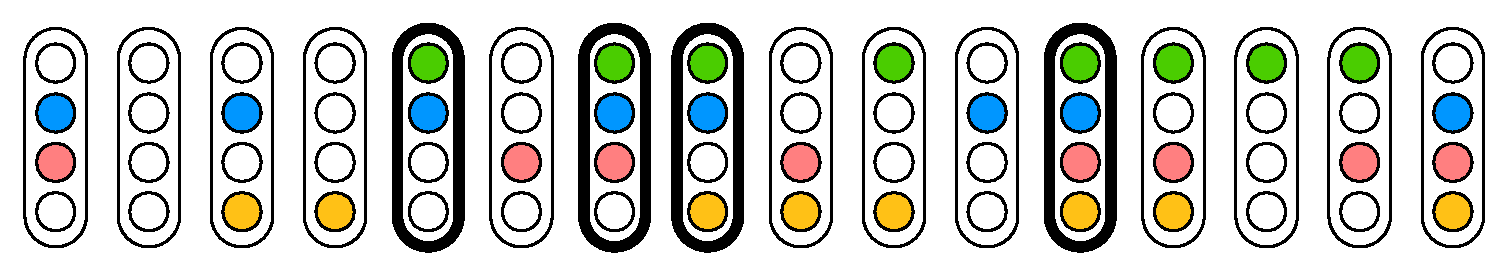
\includegraphics[scale=.335]{semaforos2.pdf}
  %\caption{Example of a concept $\con$, as shown in the experiment. Variables in $\propvars=\{x_1,x_2,x_3,x_4\}$ correspond to the presence of a  color light in the object ($x_{1}=$ green, $x_2=$ blue, $x_3=$ red, $x_4=$ orange). Items (valuations) belonging to $\con$ are highlighted with bold border. $\con$ may be described by $x_1\oand x_2$. As in a traffic light, each color is fixed to each position.}
  \caption{ESTA FIGURA SE PUEDE IR, DADO QUE ESTÁ LA NUEVA CON MÁS INFO.........Ejemplo de un concepto $\con$, como se muestra en el experimento. Cada valuación sobre $\propvars=\{x_1,x_2,x_3,x_4\}$ se representa como un `semáforo' ($x_{1}=$ verde, $x_2=$ azul, $x_3=$ rojo, $x_4=$ naranja). Que la valuación sea verdadera para $x_i$ se representa con la luz correspondiente a $x_i$ encendida; y que sea falsa, como la luz apagada. Los objetos (valuaciones) que pertenecen a $\con$ se resaltan con un borde en negrita. $\con$ puede describirse mediante $x_1\oand x_2$. Como en un semáforo, cada color está fijado siempre en la misma posición.}
  \label{semaforos}
\end{figure}

\color{magenta}
{\bf esta parte también puede ir a intro o parte 2. es común a BRM. }

%A lower bound for the complexity of a concept in a given logic corresponds to the shortest description of that concept, that is, its minimum description length (MDL).
Un límite inferior para la complejidad de un concepto en una lógica dada corresponde a la descripción más corta de ese concepto, es decir, su longitud mínima de descripción (MDL).

%The {\em size} of a formula $\varphi$ is denoted $|\varphi|$ and it is defined as the number of operators plus the number of atoms (i.e.\ possibly negated propositional symbols), that is: $|x_i|=|\lnot x_i|=1$ for $i=1\dots 4$ and $|\varphi_1*\varphi_2|=|\varphi_1|+|\varphi_2|+1$ for $*\in\{\oand,\oor,\oxor\}$. For ${\sf L} \in\{\grambool,\gramboolxor\}$ and a concept $\con$ we define the {\em minimum description length of $\con$ with respect to $\mathcal {\sf L}$} as
El {\em tamaño} de una fórmula $\varphi$ se denota como $|\varphi|$ y se define como el número de operadores más el número de átomos (símbolos proposicionales posiblemente negados), es decir: $|x_i|=|\lnot x_i|=1$ para $i=1\dots 4$ y $|\varphi_1*\varphi_2|=|\varphi_1|+|\varphi_2|+1$ para $*\in\{\oand,\oor,\oxor\}$. Para ${\sf L} \in\{\grambool,\gramboolxor\}$ y un concepto $\con$ definimos la {\em la longitud mínima de descripción de $\con$ con respecto a $\mathcal {\sf L}$} como:
$$
\mdl{\sf L}(\con)=\min\{|\varphi|\colon \varphi\in\mathcal L, \sem{\varphi}=\con\}.
$$
Como $\grambool$ es un sublenguaje de $\gramboolxor$, tenemos que $\mdl{\gramboolxor}(\con)\leq\mdl{\grambool}(\con)$ para cualquier concepto $\con$.

   \color{black}


ACA EXPLICAR LAS COSAS QUE APARECEN EN LA NUEVA FIGURA \ref{fig:notacionPRE} 

E.G., CÓMO SE REPRESENTA UNA VALUACION, UN CONCEPTO Y QUÉ SON LAS REGLAS. VER CAPTION DE FIG \ref{semaforos}, PERO ESA FIGURA SE VA.
 

\begin{figure}[t!]
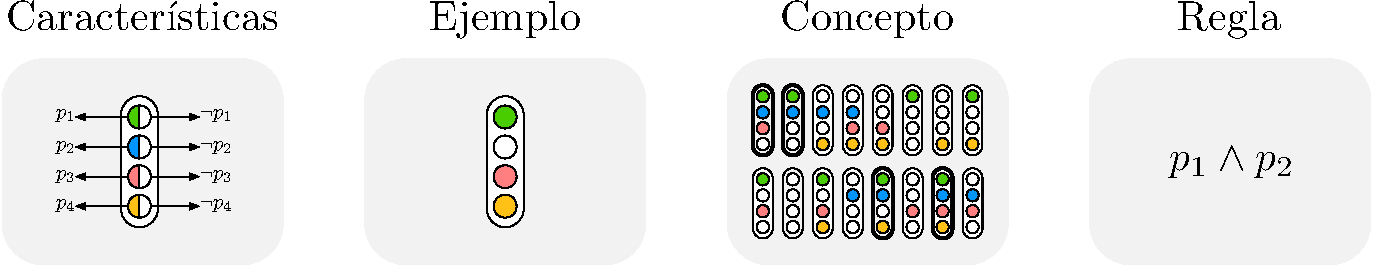
\includegraphics[scale=.6]{../figuras/pre/notacion.pdf}
\caption{FIGURA NUEVA....AGREGAR CAPTION}\label{fig:notacionPRE}
\end{figure}
\widesanti{Sergio, esta imagen es nueva. Pienso que puede dar coherencia con BRM. Puede remplazar a la figura anterior. Hay que actualizar notación en el texto y cambiar $x_i$ por $p_i$, etc. Cuando se presente la figura análoga en BRM, podes mandar un cf. a esta}


\paragraph*{Ejemplo.}El concepto $
\con=\{v\colon v(x_1)+v(x_2)=1\},
$
%which expresses that $x_1$ is true or $x_2$ is true but not both can be described in \gramboolxor as $\varphi=x_{1} \oxor x_{2}$, of length 3. In fact, one can check that this is the shortest formula compatible with $\con$, and so $\mdl{\gramboolxor}(\con)=3$. If we now switch to \grambool, we can no longer describe $\con$ as $x_{1} \oxor x_{2}$, since $\oxor$ is not part of its signature. However, in \grambool, the concept $\con$ may be described by  formula $\psi=(x_{1} \oand \neg x_{2}) \oor (x_{2} \oand \neg x_{1})$, of size 7. Since this formula has minimal size, we have that $\mdl{\grambool}(\con)=7$.
que expresa que $x_1$ es verdadero o $x_2$ es verdadero, pero no ambos, puede describirse en \gramboolxor como $\varphi=x_{1} \oxor x_{2}$, de tamaño 3. De hecho, se puede comprobar que esta es la fórmula más corta que describe a $\con$ (en el sentido de que $\sem{\varphi}=\con$), por lo que $\mdl{\gramboolxor}(\con)=3$. Si ahora cambiamos a \grambool, ya no podemos describir a $\con$ como $x_{1} \oxor x_{2}$, dado que $\oxor$ no es parte del lenguaje. Sin embargo, en \grambool, el concepto $\con$ puede describirse mediante la fórmula $\psi=(x_{1} \oand \neg x_{2}) \oor (x_{2} \oand \neg x_{1})$, de tamaño 7. Dado que esta fórmula tiene tamaño mínimo para ese concepto en \grambool, tenemos que $\mdl{\grambool}(\con)=7$.


\section{Experimento}


\renewcommand*{\arraystretch}{1.2}
   
\begin{table*}[!ht]
\vspace{-0.5cm}
\centering

\begin{tabular}{|c|l l | c | c |l l | c | c|}
\hline
                                   &
\multicolumn{2}{c|}{\textbf{Grupo objetivo}}       &
\textbf{$\mdl{\gramboolxor}(\con)$} &
\textbf{$\mdl{\grambool}(\con)$} &
\multicolumn{2}{c|}{\textbf{Grupo control}}  &
\textbf{$\mdl{\gramboolxor}(\con)$} &
\textbf{$\mdl{\grambool}(\con)$} 
 \\ \hline
\multirow{4}{*}{\parbox[t]{2mm}{\rotatebox[origin=c]{90}{\bf Entrenamiento}}} & \targeta & $x_{i}$             & 1 & 1                                                                  & \multicolumn{4}{c|}{$\longleftarrow$Ídem}                                                            \\ \cline{2-9}
                                   &\targetb& $x_{i} \oxor x_{j}$       & 3 & 7 &\controlb& $x_{i} \oor x_{j}$  & 3 & 3                                                                  \\ \cline{2-9}
                                  &\targetc & $x_{i} \oxor x_{j} \oxor x_{k}$ & 5 & 19 &\controlc& $x_{i} \oor (x_{j} \oand x_{k})$  & 5 & 5 \\ \cline{2-9}
                                  &\targetd& $x_{k} \oxor x_{l}$       & 3 & 7&\controld&$x_{k} \oor x_{l}$  & 3 & 3                                                                  \\ \hline
\multirow{2}{*}{\parbox[t]{2mm}{\rotatebox[origin=c]{90}{\bf Evaluación}}}  &\testa& $x_{i} \oand (x_{j} \oxor x_{k})$ & 5 & 9                 & \multicolumn{4}{c|}{$\longleftarrow$Ídem}                                                                                    \\ \cline{2-9}
                               &\testb& $x_{i} \oand (x_{j} \oor x_{k})$  & 5 & 5         & \multicolumn{4}{c|}{$\longleftarrow$Ídem}                                                                                            \\ \hline
\end{tabular}

\caption{Secuencia de conceptos presentados en el experimento: \targeta, \targetb, \targetc, \targetd, \testa, \testb para el grupo objetivo y  \controla, \controlb, \controlc, \controld, \testa, \testb para el grupo control. Cada concepto $\con$ está representado por una fórmula mínima $\varphi$ tal que $\sem{\varphi}=\con$. %Numbers $n/m$ on the right indicate $n=\mdl{\gramboolxor}(\con)$ and $m=\mdl{\grambool}(\con)$.
%MDL is measured as the number of operators and variables (excluding the \textit{not} operator) of the minimal formula with respect to the specified CFG.
}
\label{conceptos}
\vspace{-0.4cm}
\end{table*}


\begin{center}
\begin{table}[]\small
\begin{tabular}{|c|c||c|c|c||c|c|c|}
\hline
\textbf{}                 & \textbf{Prueba} & \textbf{\begin{tabular}[c]{@{}c@{}}Grupo\\ Objetivo\end{tabular}} & \textbf{$\mdl{\gramboolxor}$} & \textbf{$\mdl{\grambool}$} & \textbf{\begin{tabular}[c]{@{}c@{}}Grupo\\ Control\end{tabular}} & \textbf{$\mdl{\gramboolxor}$} & \textbf{$\mdl{\grambool}$} \\ \hline
\multirow{4}{*}{\parbox[t]{2mm}{\rotatebox[origin=c]{90}{Entrenamiento\ \ \ \ \ \\ \ \  }}} & 1               & \begin{tabular}[c]{@{}c@{}}\targeta \\ $x_{i}$\end{tabular}                     & 1              & 1               & \multicolumn{3}{c|}{$\longleftarrow$ ídem}                                                                           \\ \cline{2-8} 
                          & 2               & \begin{tabular}[c]{@{}c@{}}\targetb\\ $x_{i} \oxor x_{j}$\end{tabular}                     & 3              & 7               & \begin{tabular}[c]{@{}c@{}}\controlb\\ $x_{i} \oor x_{j}$\end{tabular}                    & 3              & 3               \\ \cline{2-8} 
                          & 3               & \begin{tabular}[c]{@{}c@{}}\targetc \\ $x_{i} \oxor x_{j} \oxor x_{k}$\end{tabular}                     & 5              & 19              & \begin{tabular}[c]{@{}c@{}}\controlc\\ $x_{i} \oor (x_{j} \oand x_{k})$\end{tabular}                    & 5              & 5               \\ \cline{2-8} 
                          & 4               & \begin{tabular}[c]{@{}c@{}}\targetd\\ $x_{k} \oxor x_{l}$\end{tabular}                     & 3              & 7               & \begin{tabular}[c]{@{}c@{}}\controld\\$x_{k} \oor x_{l}$\end{tabular}                    & 3              & 3               \\ \hline
\multirow{2}{*}{\parbox[t]{2mm}{\rotatebox[origin=c]{90}{Evaluación}}}     & 5               & \begin{tabular}[c]{@{}c@{}}\testa\\ $x_{i} \oand (x_{j} \oxor x_{k})$\end{tabular}                     & 5              & 9               & \multicolumn{3}{c|}{$\longleftarrow$ ídem}                                                                           \\ \cline{2-8} 
                          & 6               & \begin{tabular}[c]{@{}c@{}}\testb\\ $x_{i} \oand (x_{j} \oor x_{k})$\end{tabular}                     & 5              & 5               & \multicolumn{3}{c|}{$\longleftarrow$ ídem}                                                                           \\ \hline
\end{tabular}
\end{table}
\end{center}
\widesanti{hice esta tabla como la anterior pero con diseño para que entre. Si te gusta y la querés cambiar, adelante. Solo que antes hay que revisar que tenga los mismos datos!!!}


\widesanti{habría que unificar con BRM las $x$ con las $p$ (o no). En parte II están presentado con $p$s}

%55 participants participated in the experiment over the world wide web using the Amazon Mechanical Turk crowd sourcing platform. All were US residents over the age of 18 and had more than 95\% of past tasks successfully approved by other requesters. 44 participants completed the experiment through all the stages and declared not cheating (using pen, screenshots or a similar method to copy the answers) at the end of the experiment. Only data from these participants were used in the analyses reported below.\footnote{The learning times of all participants can be found in https://figshare.com/s/04d338adbbc4b1e83bf0.}

Un total de 55 personas participaron en el experimento a través de internet utilizando la plataforma de \textit{crowdsourcing} Amazon Mechanical Turk. Todos los participantes fueron residentes de EE.UU., mayores de 18 años y tenían más del 95\% de tareas pasadas aprobadas con éxito en la plataforma. Sólo 44 de ellos completaron todas las etapas del experimento y declararon no hacer trampas al final del experimento (se les aclaró que --aunque admitieran haber realizado anotaciones, capturas de pantalla o utilizado algún método similar-- igual serían calificados de manera positiva y recibirían su pago por haber realizado todas las etapas, pero que la información era crucial para los fines del análisis de los datos del experimento). En los análisis que se informan a continuación, sólo se utilizaron los datos de estos 44 participantes. \footnote{Los tiempos de aprendizaje de todos los participantes se pueden descargar en https://figshare.com/s/04d338adbbc4b1e83bf0.}

%Participants were divided randomly into a control group ($N=21$) and a target group ($N=23$). Both groups were presented with different sequences of six concepts. For each concept, there was a learning phase, a testing phase and a feedback phase. The average time spent in each concept was 167$\pm$20 s.e.m.\ seconds, and the average duration of the task was 21$\pm$4 s.e.m.\ minutes. After moving through the learning, testing and feedback phase of each of the six concepts, participants were asked if they used a pen or recorded the screen information in any way. They were also told that the answer to this question will not affect their payment, but that it was crucial for the experimenters to know.

Los participantes se dividieron aleatoriamente en un grupo de control ($N=21$) y en un grupo objetivo ($N=23$). A ambos grupos se les presentaron diferentes secuencias de seis conceptos. Para cada concepto, hubo una fase de {\em aprendizaje} y una fase de {\em entrenamiento-feedback}. La media del tiempo empleado en cada concepto fue de 167$\pm$20 s.e.m.\ segundos, y la duración promedio de la tarea fue de 21$\pm$4 s.e.m.\ minutos. 

%During the learning phase, all 16 items were presented in the screen (in random order), and items belonging to the concept were identified with bold boundaries, as shown in  Fig.~\ref{semaforos}. Participants were told that only the items with bold boundaries were `blickets' (or `tufas', etc.: we used different words for each concept in the sequence), and asked them to try to identify what a blicket was. During the testing phase, the 16 items were shuffled in the screen, and participants were asked to click on items that were blickets. If they made mistakes after submitting their answer, they were directed to the feedback phase, in which items that were incorrectly classified were indicated with a red cross. After having studied the feedback, participants were redirected to the testing screen, where items were reshuffled. When every item was correctly classified, participants were asked to give a verbal description of the concept and then continued on to the following concept after a resting period. We characterize the subjective difficulty of each concept as the time the participant spent in learning, testing and feedback phases for that concept (excluding the time spent in the verbal description).

Durante la fase de {\em aprendizaje}, los 16 elementos (correspondientes a las 16 valuaciones posibles sobre $\propvars$) se presentaban en la pantalla (en orden aleatorio), y los elementos pertenecientes al concepto se identificaban con los bordes resaltados, como se muestra en la Figura~\ref{semaforos}. A los participantes se les decía que sólo los elementos resaltados eran `blickets' (o `tufas', etc.: usamos diferentes palabras para cada concepto en la secuencia), y se les pedía que intentaran identificar qué era un `blicket'. Durante la etapa de {\em entrenamiento}, los 16 ítems eran mezclados y mostrados en la pantalla, y se les pedía que hicieran clic en los elementos que eran blickets. Si al enviar su respuesta cometían errores, se los dirigía a la pantalla de {\em feedback} donde los elementos que se clasificaron incorrectamente se marcaban con una cruz roja. Luego de haber estudiado la respuesta, los participantes eran redirigidos a la pantalla de prueba, donde los elementos eran nuevamente mezclados y mostrados en pantalla para su selección. Esto se repetía hasta que los participantes seleccionaran correctamente todos los elementos. Una vez que la selección era correcta, se les pedía que dieran una descripción verbal del concepto y luego continuaban con el siguiente concepto tras un breve período de descanso. Caracterizamos la dificultad subjetiva de cada concepto como el tiempo que un participante pasó en las fases de {\em aprendizaje} y e {\em entrenamiento-feedback} para cada concepto (excluyendo el tiempo dedicado a la descripción verbal). Una visión esquemática del experimento se puede ver en la Figura~\ref{fig:experimentoPRE}.

\begin{figure}
\begin{center}
  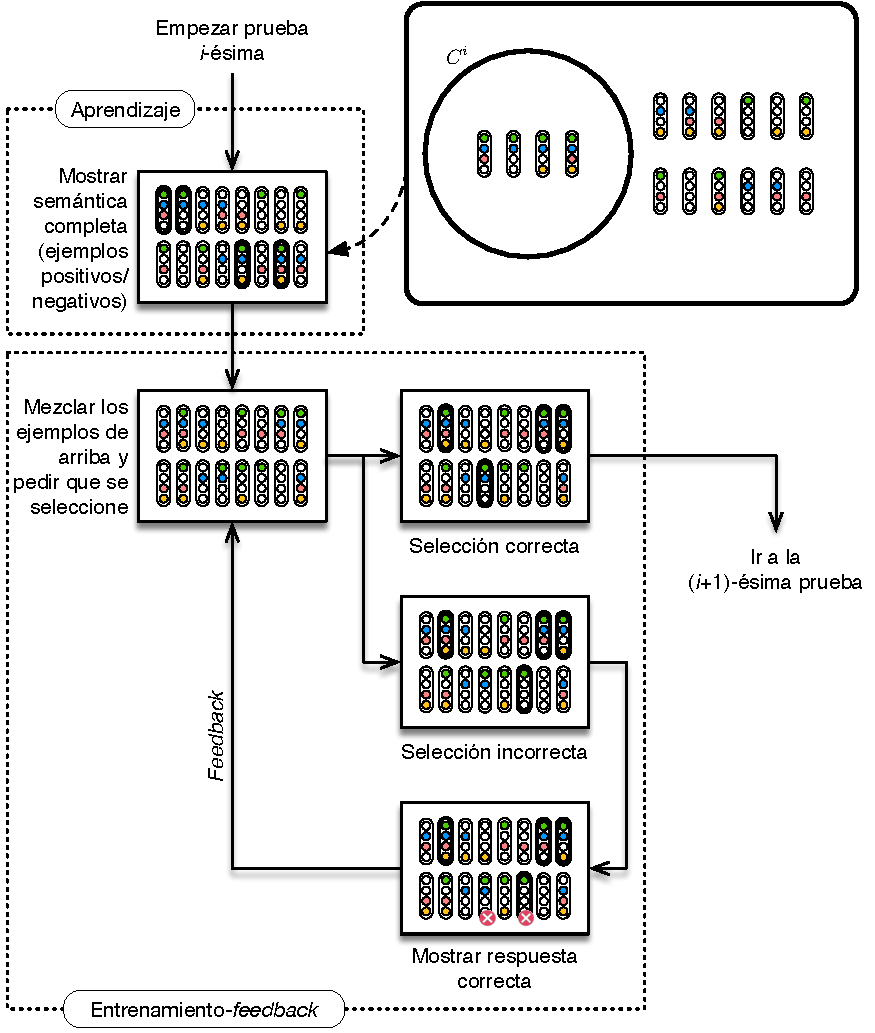
\includegraphics[scale=1]{../figuras/pre/experimento_PRE.pdf}
\end{center}\caption{El esquema de funcionamiento del experimento.}\label{fig:experimentoPRE}
\end{figure}
\widesanti{Sergio, esta figura es nueva. Es una adaptación de la de BRM, más simple y con los ejemplos de semáforos. Pienso que puede dar más coherencia a la tesis. Podés confrontarla desde el capítulo de BRM y decir que en BRM es más complejo: (a) mostramos semantica INCOMPLETA (b) hay 2 conceptos en vez de 1 y (c) hay una etapa de GENERALIZACION}

%Both groups (target and control), were exposed to 6 concepts. The second, third and fourth concepts are {\em training} concepts, and were different between both groups. The last two concepts are the {\em test} concepts, and were the same for both groups. The first concept was the trivial concept $x_i$ for both groups, which was aimed to get participants started in the task. Importantly, variables (i.e. color lights inside objects in Fig.~\ref{semaforos}) were randomized for every concept, so paying selective attention to a specific variable across subsequent concepts was not beneficial for learning the concept sequence.

Ambos grupos (objetivo y control), fueron expuestos a 6 conceptos. El segundo, tercero y cuarto concepto son los conceptos de {\em entrenamiento} y fueron diferentes para cada grupo. Los últimos dos conceptos son los conceptos de {\em evaluación}, y fueron los mismos para ambos grupos. El primer concepto fue el concepto trivial $x_i$ para ambos grupos, cuyo objetivo fue que los participantes se familiarizaran con la tarea. Es importante destacar que las variables (es decir, las luces de color dentro de los objetos en la Figura~\ref{semaforos}) fueran seleccionadas de manera aleatoria para cada concepto, por lo que prestar atención selectiva a una variable específica para los conceptos siguientes no era beneficioso para aprender la secuencia de conceptos.

%As shown in Table~\ref{conceptos}, we presented the target group with training concepts which are succinctly described when $\oxor$ is part of the language, but necessarily described with lengthier formulas if $\oxor$ is absent; more technically, concepts for which $\mdl{\gramboolxor}$ is much smaller than $\mdl{\grambool}$. We also corroborated that for \targetb, \targetc, \targetd and \testa the number of formulas in $\gramboolxor$ with length strictly smaller than $\mdl{\grambool}$ was at least 10 times greater than the number of formulas in $\grambool$ with length equal to $\mdl{\grambool}$.

Como se muestra en la Tabla~\ref{conceptos}, presentamos al grupo objetivo conceptos de entrenamiento que se describen sucintamente cuando $\oxor$ es parte del lenguaje, pero que necesariamente se describen con fórmulas más largas si $\oxor$ está ausente; más técnicamente, conceptos para los que $\mdl{\gramboolxor}$ es mucho más pequeño que $\mdl{\grambool}$. También corroboramos que para \targetb, \targetc, \targetd y \testa, el número de fórmulas en $\gramboolxor$ con una longitud estrictamente menor que $\mdl{\grambool}$ era al menos 10 veces mayor que el número de fórmulas en $\grambool$ con longitud igual a $\mdl{\grambool}$.

%Participants in the control group, on the other hand, experienced a sequence of concepts that could be easily described using the language given by \grambool. After these training concepts, both groups were presented with the same pair of test concepts: one which could be only succinctly described in \gramboolxor, and one for which the MDL did not depend on the underlying language \gramboolxor or \grambool. We compared learning times between the two groups for these last two concepts.

Los participantes en el grupo control, por otro lado, experimentaron una secuencia de conceptos que podía describirse fácilmente usando el lenguaje dado por \grambool. Después de estos conceptos de entrenamiento, a ambos grupos se les presentó el mismo par de conceptos de evaluación: uno que sólo podía ser descrito sucintamente en \gramboolxor, y uno para el que el MDL no dependía si el lenguaje subyacente era \gramboolxor o \grambool. Comparamos los tiempos de aprendizaje entre los dos grupos para estos dos últimos conceptos.


%As shown in Table~\ref{conceptos}, training concepts for the target (xor) group were: $x_{i}$, $x_{i} \oxor x_{j}$, $x_{i} \oxor x_{j} \oxor x_{k}$, and $x_{k} \oxor x_{l}$, called \targeta, \targetb, \targetc and \targetd respectively. Training concepts for the control group were: $x_{i}$, $x_{i} \oor x_{j}$, $x_{i} \oor (x_{j} \oand x_{k})$, and $x_{k} \oor x_{l}$ called \controla, \controlb, \controlc and \controld respectively. We use the indexes \textit{i, j, k, l} instead of numbers because variables were randomized in each trial. $x_{i}$ could stand for $x_1$, $x_2$, $x_3$ or $x_4$, that is, for any of the four colors. After these four concepts, both groups were presented with the same test concepts: $x_{i} \oand (x_{j} \oxor x_{k})$, and $x_{i} \oand (x_{j} \oor x_{k})$, called \testa and \testb respectively.

Como se muestra en la Tabla~\ref{conceptos}, los conceptos de entrenamiento para el grupo objetivo (xor) fueron: $x_{i}$, $x_{i} \oxor x_{j}$, $x_{i} \oxor x_{j} \oxor x_{k}$, y $x_{k} \oxor x_{l}$, llamados \targeta, \targetb, \targetc y \targetd respectivamente. Los conceptos de entrenamiento para el grupo control fueron: $x_{i}$, $x_{i} \oor x_{j}$, $x_{i} \oor (x_{j} \oand x_{k})$, y $x_{k} \oor x_{l}$ llamados \controla, \controlb, \controlc y \controld respectivamente. Usamos los índices \textit{i, j, k, l} en lugar de números porque las variables fueron elegidas de manera aleatoria en cada ensayo. Así, $x_{i}$ podría representar $x_1$, $x_2$, $x_3$ o $x_4$, es decir, cualquiera de los cuatro colores. Después de estos cuatro conceptos, a ambos grupos se les presentaron los mismos conceptos de evaluación: $x_{i} \oand (x_{j} \oxor x_{k})$, y $x_{i} \oand (x_{j} \oor x_{k})$, llamados \testa y \testb respectivamente.

%Choosing which concepts to show the target group in order for them to `learn' the $\oxor$ operator is critical in our experiment. Crucially, the learner must have an option between two alternatives that describe the concept: one that is succinct but uses $\oxor$, or necessarily a much longer one in the absence of $\oxor$. In other words, these concepts must be compatible with short logical formulas if and only if we take \gramboolxor as the language of description. To ensure that this was the case, we enumerated, for each concept, all formulas compatible with it and produced by the \grambool and \gramboolxor grammars up to length 19. For all training concepts of the target group, the shortest compatible formula without $\oxor$ is much longer than the shortest compatible formula with $\oxor$. This is shown in Table\ref{conceptos}.

Elegir qué conceptos mostrar al grupo objetivo para que `aprendan' el operador $\oxor$ es una parte clave de nuestro experimento. El sujeto debe tener una opción entre dos alternativas que describan el concepto: una que es sucinta pero usa el operador $\oxor$, o una que sea necesariamente mucho más larga en ausencia del $\oxor$. En otras palabras, estos conceptos deben ser compatibles con fórmulas lógicas cortas si y sólo si tomamos \gramboolxor como el lenguaje de descripción. Para asegurarnos de que este fuera el caso, enumeramos, para cada concepto, todas las fórmulas compatibles con él que se puedan producir con las gramáticas \grambool y \gramboolxor hasta la longitud 19. Para todos los conceptos de entrenamiento del grupo objetivo, la fórmula compatible más corta sin $\oxor$ es mucho más larga que la fórmula compatible más corta con $\oxor$. Esto se muestra en la Tabla~\ref{conceptos}.

%\section{Model-Free Results}
\section{Resultados sin modelo}

%We measure the subjective difficulty of a given concept as the total time needed by the participant to successfully encode the concept, which indicates that they can reliably express which exemplars belong to the concept and which do not.

Medimos la dificultad subjetiva de un concepto dado como el tiempo total que necesita el participante para codificar con éxito el concepto, lo que indica que pueden expresar qué ejemplares perteneces al concepto y cuáles no.


%Participants from the target group spent almost half the time than participants from the control group in \testa, which could be succinctly described only in \gramboolxor ($111\pm16$ s.e.m.\ seconds versus $214\pm37$ s.e.m.\ seconds, a two-sample t-test reveals $t_{42}=2.6$, $P<0.01$), as shown in Fig.~\ref{model free} (a). We also found that the control group learned much faster \testb ($143\pm14$ s.e.m.\ seconds for the target group versus $76\pm10$ s.e.m.\ seconds for the control group, $t_{42}=3.5$, $P<0.01$). A mixed ANOVA with \testa-\testb as within subject factor and target-control groups as between subject factor reveals a strong interaction between group and \testa-\testb ($F=15.3$, $P<0.001$), indicating that the differences in learning times for \testa and \testb were very different between the two groups.

Los participantes del grupo objetivo pasaron casi la mitad del tiempo que los participantes del grupo control en \testa, que podía describirse sucintamente sólo en \gramboolxor ($111\pm16$ s.e.m.\ segundos contra $214\pm37$ s.e.m.\ segundos, una prueba t para dos muestras revela $t_{42}=2.6$, $P<0.01$), como se muestra en la Figura.~\ref{model free} (a). También encontramos que el grupo de control aprendió mucho más rápido \testb ($143\pm14$ s.e.m.\ segundos para el grupo objetivo contra $76\pm10$ s.e.m.\ segundos para el grupo control, $t_{42}=3.5$, $P<0.01$). Un ANOVA mixto con \testa-\testb como factor dentro de los sujetos y grupos objetivo-control como factor entre sujetos revela una fuerte interacción entre el grupo y \testa-\testb ($F=15.3$, $P<0.001$), lo que indica que las diferencias en el aprendizaje de los tiempos para \testa y \testb fueron muy diferentes entre los dos grupos.

%The target group encoded \testa more efficiently than the control group. We propose that the control group expected to find in \testa and \testb structures that could be easily built in \grambool. The target group, on the other hand, became biased towards the $\oxor$ structure, and they expected to find it in \testa and \testb. This caused \testa to be encoded more rapidly by the target group and \testb more rapidly by the control group. Assuming that the subjective difficulty of learning a concept is proportional to the complexity of its internal representation, we conclude that after exposure to the training concepts, participants in the target group represented the $\oxor$ more efficiently than the control group, and expected to find this structure in \testa and \testb.

El grupo objetivo codificó \testa de manera más eficiente que el grupo control. Proponemos que el grupo control esperaba encontrar en \testa y \testb estructuras que pudieran ser fácilmente construidas en \grambool. El grupo objetivo, por otro lado, se inclinó hacia la estructura $\oxor$, y esperaban encontrarlo en \testa y \testb. Esto provocó que \testa se codificara más rápido por el grupo objetivo y \testb más rápido por el grupo control. Suponiendo que la dificultad subjetiva de aprender un concepto es proporcional a la complejidad de su representación, llegamos a la conclusión que -después de la exposición a los conceptos de entrenamiento- los participantes en el grupo objetivo representaron el $\oxor$ de manera más eficiente que el grupo control, y esperaban encontrar esta estructura en \testa y \testb.



\begin{figure}[t!]
      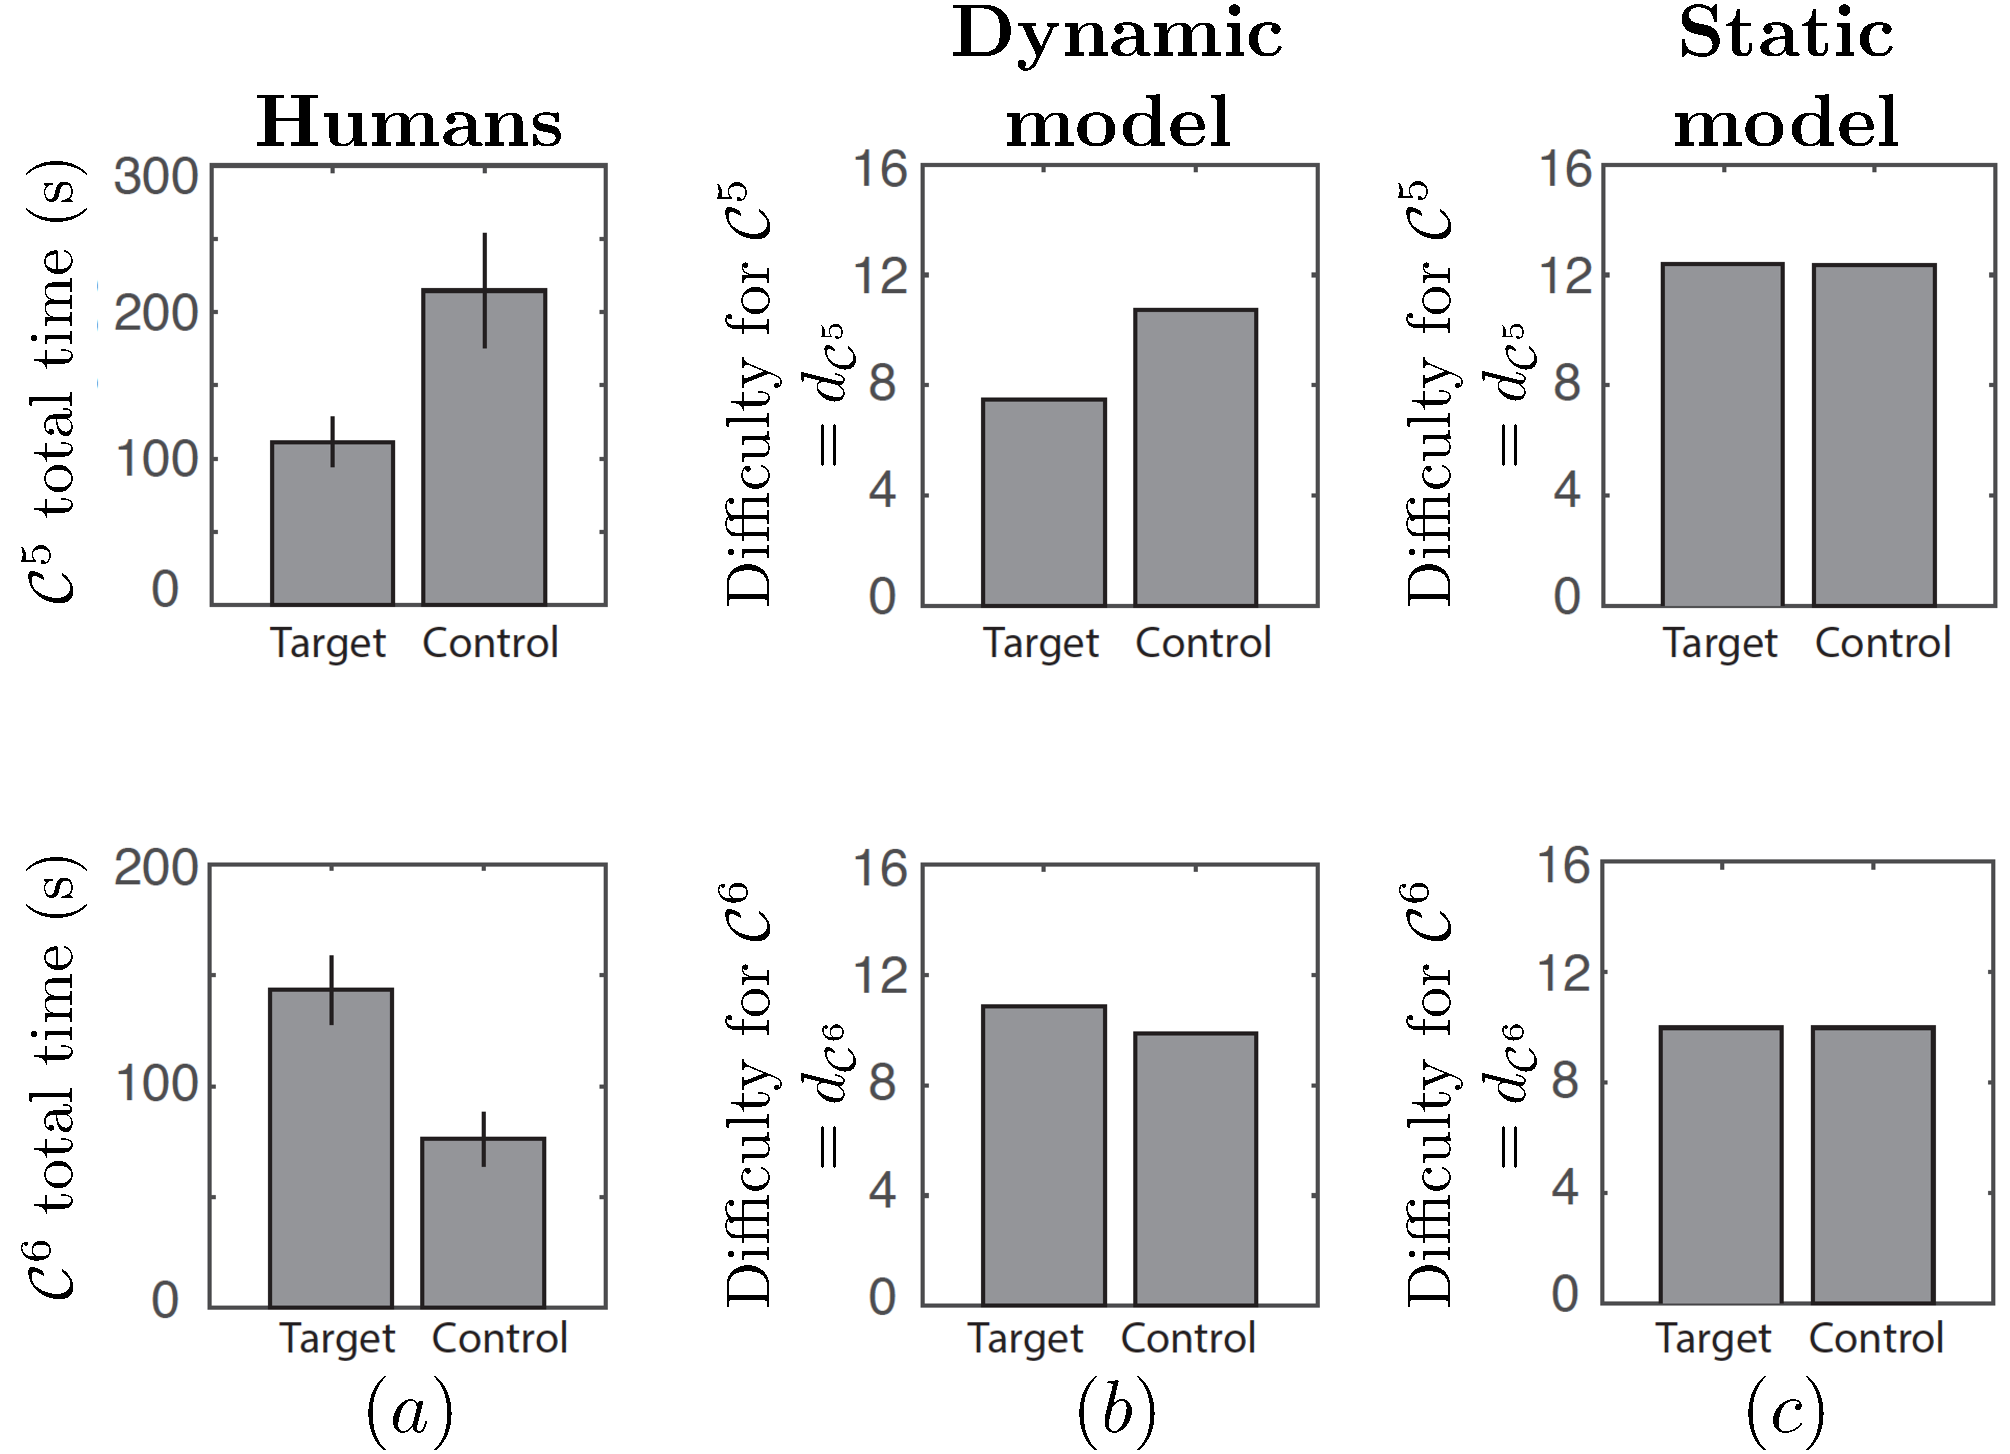
\includegraphics[scale=0.25]{model_free-3.pdf}
      \centering
      %\caption{Concept learning time $(a)$ and difficulty predicted $(b)$, $(c)$ for the two test concepts (\testa and \testb). Error bars are s.e.m.\ across subjects.}
      \caption{Tiempo de aprendizaje del concepto $(a)$ y dificultad pronosticada $(b)$, $(c)$ para los dos conceptos de evaluación (\testa y \testb). Las barras de error son s.e.m.\ entre los sujetos}
      \label{model free}
   \end{figure}
   
\section{Modelo}

%When presented with a concept (e.g.~Fig.~\ref{semaforos}), our model generates logical formulas and evaluate them to true or false for that concept, keeping the formula only if it is true. To generate formulas, the model uses a symbolic language in which each rule (symbols and operators) is associated with a probability of being used. The probability of generating a formula is proportional to the product of the probabilities of the rules required for building it, and therefore it decreases exponentially with its length. Furthermore, if one of the rules has a very low probability of being used, formulas that require it will also have very low probability.


Cuando se le presenta un concepto (por ejemplo, Figura~\ref{semaforos}), nuestro modelo genera fórmulas lógicas y las evalúa como verdadero o falso para ese concepto, manteniendo la fórmula sólo si es verdadera. Para generar fórmulas, el modelo utiliza un lenguaje simbólico en el que cada regla de producción (símbolos y operadores) está asociado con una probabilidad de ser utilizado. La probabilidad de generar una fórmula es proporcional al producto de las probabilidades de las reglas requeridas para construirla y, por lo tanto, disminuye exponencialmente con su longitud. Además, si una de las reglas tiene una probabilidad muy baja de ser utilizada, las fórmulas que la requieran también tendrán una muy baja probabilidad.

%The \textit{Static model} maintains the rules' probabilities fixed throughout the concept sequence (the 6 concepts in Table~\ref{conceptos}). The \textit{Dynamic model} updates the probabilities after each concept, in order to minimize the expected description length of future concepts, assuming they have similar structure to the concepts learnt so far. We include in this model the $\oxor$ rule a priori in the language, but with vanishing probability of being used. Changes in this probability can be analogously interpreted as the probability that a rational agent without the compiled symbol a priori decides to add the compiled expression as a new primitive into her language. %This means that our model will fit somewhere between the computational and the algorithmic level of analysis by Marr's~\cite{marr1979computational,griffiths2015rational}. It can explain algorithmically how learning occurs, however, adding a new primitive is not modeled entirely at this level. The vanishing probability analogy is sufficient to make the new primitive be highly unlikely to be used without exposure and to allow it to emerge after concepts. Still, it does not explain --at an algorithmic level-- how any new primitive can arise, leaving the mechanics of the language change between the computational and algorithmic level.

El \textit{modelo estático} mantiene las probabilidades de las reglas fijas a lo largo de la secuencia de conceptos (los 6 conceptos de la Tabla~\ref{conceptos}). El \textit{modelo dinámico} actualiza las probabilidades después de cada concepto, con el fin de minimizar la longitud de descripción esperada de conceptos futuros, asumiendo que tienen una estructura similar a los conceptos aprendidos hasta ahora. Incluimos en este modelo el operador $\oxor$ a priori en el lenguaje, pero con una probabilidad de ser utilizado muy baja. Cambios en esta probabilidad se pueden interpretar análogamente como la probabilidad de que un agente racional sin el símbolo compilado a priori decida agregar la expressión compilada como un nuevo operador en su lenguaje.


\subsection{Modelo estático}

\newcommand{\form}{\varphi}
\sergio{esto se explica en PlosOne}
%Under the \lot assumption,  given a concept $\con$ (e.g.\ Fig.~\ref{semaforos}), the probability that an agent uses formula $\form$ to explain this concept is defined by Bayes theorem: 
Bajo la hipótesis de \lot,  dado un concepto $\con$ (por ejemplo, \ Figura.~\ref{semaforos}), la probabilidad de que un agente use la fórmula $\form$ para explicar el concepto está definida por el teorema de Bayes: 
$$
P(\form\mid \con) \propto P(\con\mid \form)P(\form).
\label{Bayes fix}
$$
% \begin{equation}
% P(\form\mid \con) \propto P(\con\mid \form)P(\form).
% \label{Bayes fix}
% \end{equation}
%
%The likelihood $P(\con\mid \form)$ of a logical statement $\form$ can be simply defined as 1 if $\sem{\form}=\con$ and 0 otherwise. In other words, for any given concept, only explanations that describe this concept are considered as possible explanations. The likelihood term has been defined more flexibly in the literature~\cite{goodman2008rational,piantadosi2016logical}, allowing for mislabeled elements. We keep this simpler definition in order to reduce the number of free parameters of the model, as we do not intend to account for mislabeling errors in our experiment.

La función de verosimilitud $P(\con\mid \form)$ de un enunciado lógico $\form$ se puede definir simplemente como 1 si $\sem{\form}=\con$ y 0 en caso contrario. En otras palabras, para cualquier concepto dado, sólo las explicaciones que describen este concepto se consideran como posibles explicaciones. Se ha definido la función de verosimilitud de manera más flexible en la literatura~\cite{goodman2008rational,piantadosi2016logical}, permitiendo elementos mal etiquetados. Mantenemos esta definición más simple para reducir el número de parámetros libres del modelo ya que no pretendemos tener en cuenta los errores de etiquetado en nuestro experimento. \sergio{esto se explica en PlosOne}

%The prior $P(\form)$ is defined by augmenting the context-free grammars shown in Fig.~\ref{PCFG} into a probabilistic context-free grammars (PCFG). In the PCFG, each rule has associated a parameter indicating the probability of using that rule. A PCFG can be used to produce logical statements similar to a CFG. Each non-terminal remaining in the statement is expanded using a rule of the PCFG with probability proportional to that rule's associated parameter, until no non-terminals remain in the statement. 

La probabilidad a priori $P(\form)$ se define aumentando las gramáticas libre de contexto (CFG) que se muestran en la Figura~\ref{PCFG} en gramáticas probabilísticas libres de contexto (PCFG). En la PCFG, cada regla tiene asociado un parámetro que indica la probabilidad de utilizar esa regla. Se puede utilizar una PCFG para producir enunciados lógicos de manera similar a una CFG. Cada no terminal en la expresión es expandido usando una regla de la PCFG con probabilidad proporcional al parámetro asociado a la regla hasta que no queden no terminales en la expresión. \sergio{esto se explica en PlosOne}

%We assume that the probability that a subject uses formula $\form$ to explain concept $\con$ is proportional to the posterior $P(\form \mid \con)$, and the subjective difficulty $d_\con$ of a concept $\con$ to a participant is proportional to the length of the formula that the participant is using to explain that concept. However, there is no way to know directly which internal formula $\form$ the participant is using (and therefore we do not know $|\form|$). Hence, the most parsimonious approach is to consider the entire posterior distribution $\textbf{P}(\form \mid \con)$ over possible formulas.\footnote{This is equivalent to the Sampling Hypothesis described in~\cite{denison2013rational}, by which participants represent distributions through samples. Similar results are obtained if each participant carries entire probability distributions.}

Suponemos que la probabilidad que un sujeto utilice la fórmula $\form$ para explicar el concepto $\con$ es proporcional a la probabilidad a posteriori $P(\form \mid \con)$, y que la dificultad subjetiva $d_\con$ de un concepto $\con$ para un participante es proporcional a la longitud de la fórmula que el participante está usando para explicar ese concepto. Sin embargo, no hay forma de saber directamente qué fórmula interna $\form$ está utilizando el participante (y por tanto no sabemos $|\form|$). De ahí, el enfoque más parsimonioso consiste en considerar la distribución a posteriori $\textbf{P}(\form \mid \con)$ de manera completa sobre todas las posibles fórmulas.\footnote{Esto es equivalente a la hipótesis de muestreo descripta en~\cite{denison2013rational}, por la cual los participantes representan distribuciones a través de muestras. Se obtienen resultados similares si cada participante traslada la distribución de probabilidad completa} \sergio{no estoy seguro de cómo explicarlo}

%Given a concept $\con$, the expected length $E_\con$ of the formulas used by the participant is simply
Dado un concepto $\con$, la longitud esperada $E_\con$ de las fórmulas utilizadas por el participante es simplemente:
%
 \begin{equation}
E_\con=\sum_{\sem{\form}=\con} |\form| \ P(\form \mid \con),
 \label{expected length}
 \end{equation}
%
%where the sum is over all formulas $\varphi$ compatible with $\con$. We  define the difficulty $d_\con$ of a concept experienced by the participant  as $$d_\con \propto E_\con + \alpha N_\con,$$
donde la suma es sobre todas las fórmulas $\varphi$ compatibles con $\con$. Definimos la dificultad $d_\con$ de un concepto experimentado por un participante como $$d_\con \propto E_\con + \alpha N_\con,$$
%
% \begin{equation}
%d_\con \propto E_\con + \alpha N_\con,
% \label{length}
% \end{equation}
%
%where we added a term that accounts for the cardinality of the concept: $N_\con$ is the cardinality of the concept or its complement, the one being smaller, i.e.\ $N_\con=\min \{ \#\con, \#\overline \con\}$ (e.g.\ $N_\con=4$ for the concept $\con$ of  Fig.~\ref{semaforos}), and $\alpha$ is a free parameter fitted globally for all concepts and participants to its maximum likelihood value of 0.9. In this way, we remove the asymmetry between positive and negative examples, while accounting for the toil taken by considering a larger number of items simultaneously.
donde agregamos un término que da cuenta de la cardinalidad del concepto: $N_\con$ es la cardinalidad del concepto o su complemento, el que sea más pequeño, es decir, i.e.\ $N_\con=\min \{ \#\con, \#\overline \con\}$ (por ejemplo, \ $N_\con=4$ para el concepto $\con$ de la Figura~\ref{semaforos}), y $\alpha$ es un parámetro libre ajustado globalmente para todos los conceptos y participantes hasta su valor de máxima verosimilitud: 0.9. De esta manera, eliminamos la asimetría entre ejemplos positivos y negativos, mientras se sigue contabilizando el esfuerzo que lleva considerar un número más grande de elementos de manera simultánea.

%In practice, to approximate $E_\con$ for each concept $\con$, we calculated the posterior probability $P(\form\mid \con)$ of all compatible formulas $\form$s up to size 19 with $P(\form\mid \con)$ and then use ~\eqref{expected length}. Since the space of all possible $\form$s grows exponentially with $|\form|$, normative procedures for estimating $P(\form\mid \con)$ in this space involve stochastic search algorithms. However, in our case, we were able to exhaustively enumerate and calculate the posterior probability of \textit{all} formulas generated by the PCFG up to a sufficiently high size $M$ such that all formulas with $|\form|>M$ have vanishing probabilities when compared to shorter compatible formulas for the current concept (because the prior $P(\form)$ decreases exponentially with the size of the formula).

En la práctica, para aproximar $E_\con$ para cada concepto $\con$, calculamos la probabilidad a posteriori $P(\form\mid \con)$ de todas las fórmulas compatibles $\form$s hasta longitud 19 con $P(\form\mid \con)$ y luego utilizamos ~\eqref{expected length}. Dado que el espacio de todas las posibles $\form$s crece exponencialmente con$|\form|$, los procedimientos normativos para estimar $P(\form\mid \con)$ en este espacio implican algoritmos de búsqueda estocásticos. Sin embargo, en nuestro caso, pudimos enumerar y calcular exhaustivamente la probabilidad a posteriori de todas las fórmulas generadas por la PCFG hasta un nivel suficientemente alto de longitud $M$ tal que todas las fórmulas con $|\form|>M$ tienen probabilidades insignificantes en comparación con las fórmulas compatibles más cortas para el concepto actual (porque la probabilidad a priori $P(\form)$ decrece exponencialmente con la longitud de la fórmula).

\subsection{Modelo dinámico}

%Up to this point, we assumed that, given a concept $\con$, the posterior distribution over formulas $P(\form\mid \con)$ was independent of the other concepts presented in the sequence. However, if the \lot (i.e. the PCFG) updates with experience, the prior $P(\form)$ in $P(\form\mid \con)$ will change, and so will $E_\con$ in \eqref{expected length} and finally the subjective difficulty $d_\con$. Therefore, $d_\con$ will depend on the sequence of concepts that were previously presented to the participant.

Hasta este punto asumimos que, dado un concepto $\con$, la distribución a posteriori sobre las fórmulas $P(\form\mid \con)$ era independiente de los conceptos presentados en la secuencia. Sin embargo, si el \lot (es decir, la PCFG) se actualiza con la experiencia, la probabilidad a priori $P(\form)$ en $P(\form\mid \con)$ cambiará, al igual que $E_\con$ en \eqref{expected length} y finalmente también la dificultad subjetiva $d_\con$. Por lo tanto, $d_\con$ dependerá de la secuencia de conceptos que se presentaron previamente al participante.

En otras palabras, dado que ahora $P(\form)$ depende de la secuencia de conceptos observada por el participante, en lugar de $P(\form\mid \con)$, tendremos $$P(\form\mid \con^{t},\dots,\con^{1}) \propto P(\con^{t}\mid \form)P(\form\mid \con^{1},\dots,\con^{t-1})$$, 
% \begin{equation}
% P(\form\mid \con^{t}) \propto P(\con^{t}\mid \form)P(\form\mid \con^{1},\dots,\con^{t-1}),
% \label{Bayes}
% \end{equation}
%
%where $\con^{t}$ is the concept presented at trial~$t$, and $P(\form\mid \con^{1},\dots,\con^{t-1})$ depends on the state of the PCFG at trial $t$, which in turn depends on how the PCFG gets updated from trial to trial.
donde $\con^{t}$ es el concepto presentado en la tarea~$t$, y $P(\form\mid \con^{1},\dots,\con^{t-1})$ depende del estado de la PCFG en la tarea $t$, que a su vez depende de cómo se actualiza la PCFG entre cada tarea.

%Intuitively, the update process increases the probability of using a certain rule in the PCFG accordingly to how useful this rule was to compress compatible formulas for the concepts previously learned in the same domain. Specifically, we model the update process in a normative manner: the probability of using a rule of the PCFG at trial $t$ is equal to the Bayesian posterior probability that this rule will enable the learner to find compressed explanations at trial $t$, according to how useful it was to compress explanations in trials $1,\dots,t-1$.

Intuitivamente, el proceso de actualización aumenta la probabilidad de utilizar una determinada regla en la PCFG de acuerdo con la utilidad de esa regla para comprimir fórmulas compatibles para conceptos aprendidos previamente en el mismo dominio. Específicamente, modelamos el proceso de actualización de manera normativa: la probabilidad de utilizar una regla de la PCFG en la tarea $t$ es igual a la probabilidad a posteriori de que esta regla permita al sujeto encontrar explicaciones comprimidas en la tarea $t$, de acuerdo con la utilidad de comprimir explicaciones en las tareas $1,\dots,t-1$.

%To formalize the update of the PCFG, we define $P(\form)$ similarly to~\cite{goodman2008rational}. Specifically, the prior probability of a logical statement at trial $t$ in the concept sequence uses a single Dirichlet-multinomial for the set of rule expansions. The Dirichlet is parameterized by a set of positive real numbers $D_{i}^{t}$, one for each rule $i$ in the PCFG, which in turn determine the probability of using rule $i$ at trial $t$: a higher $D_{i}$ indicates a higher probability of using rule $i$.

Para formalizar la actualización de la PCFG, definimos $P(\form)$ de manera similar a~\cite{goodman2008rational}. Específicamente, la probabilidad a priori de una expresión lógica en la tarea $t$ en la secuencia de conceptos usa una Dirchlet multinomial para el conjunto de reglas. La distribución Dirchlet está parametrizada por un conjunto de números reales positivos $D_{i}^{t}$, uno por cada regla $i$ en la gramática, que a su vez determinan la probabilidad de utilizar la regla $i$ en la tarea $t$: una $D_{i}$ más alta indica una mayor probabilidad de utilizar la regla$i$.

%The prior is specified by the set Dirichlet parameters $\textbf{D}^{0}$ with which we start the experiment ($\textbf{D}^{0}$ represents a vector containing the prior parameters of all rules in the grammar at trial 0). In our experiment, we set the prior Dirichlet parameters of all rules equal to 1, and the parameter of the rule that expands the target operator to a value several orders of magnitude smaller ($\approx 10^{-4}$). This means that the target operator was practically absent at the beginning of the experiment, but it was technically possible to `learn it' by increasing its probability as the experiment developed.

La probabilidad a priori está especificada como el conjunto de parámetros de la Dirichlet $\textbf{D}^{0}$ con el que iniciamos el experimento ($\textbf{D}^{0}$ representa un vector que contiene los parámetros a priori de todas las reglas para la tarea 0). En nuestro experimento, establecemos los parámetros a priori de todas las reglas en 1, excepto por el de la regla que expande el operador objetivo $\oxor$ que está establecido con un valor varios órdenes de magnitud menor ($\approx 10^{-4}$). Esto significa que el operador objetivo está prácticamente ausente al comienzo del experimento, pero que es técnicamente posible `aprenderlo' si se aumenta su probabilidad a medida que se desarrolla el experimento.

%Under the Dirichlet model, the prior $P(\form\mid \con^{1},\dots,\con^{t-1})$ can be rewritten using the Dirichlet parameters as $P(\form\mid\textbf{D}^{t})$. Therefore, to know how $P(\form\mid \con)$ updates from trial to trial, we only need to know how $\textbf{D}$ updates from trial to trial.

Bajo el modelo de Dirichlet, la probabilidad a priori $P(\form\mid \con^{1},\dots,\con^{t-1})$ se puede reescribir utilizando los parámetros de la Dirichlet como $P(\form\mid\textbf{D}^{t})$. Por lo tanto, para saber cómo se actualiza $P(\form\mid \con)$ entre cada tarea, sólo necesitamos saber cómo $\textbf{D}$ se actualiza entre cada tarea.

%The Dirichlet parameter of rule $i$ at trial $t+1$ is equal to its parameter at trial $t$ plus the amount of times the production $i$ was used in generating all formulas compatible with the concept at trial $t$ (we note $M_{i}(\form)$ as the number of times that rule $i$ is used in generating formula $\form$), weighted by each formula's posterior probability at trial $t$:

El parámetro Dirichlet de la regla $i$ en la tarea $t+1$ es igual al parámetro en la tarea $t$ más la cantidad de veces que se utilizó la regla $i$ para generar todas las fórmulas compatibles con el concepto en la tarea $t$ (definimos a $M_{i}(\form)$ como el número de veces que la regla $i$ es usada para generar la fórmula $\form$), ponderada por la probabilidad a posteriori de cada fórmula en la tarea $t$:
 \begin{equation}
 D_{i}^{t+1}=D_{i}^{t}+\sum_{\sem{\form}=\con^t} P(\form\mid \textbf{D}^{t}) \ M_{i}(\form).
 \label{Dirichlet}
 \end{equation}
 %
%This Bayesian learning mechanism increases the probability of using rules that allow concepts to be succinctly described. This happens because these formulas have higher probability $P(\form\mid \textbf{D})$ than longer formulas, so the Dirichlet parameters of the rules that build these formulas increase more strongly than those of the rules that build longer formulas.   

Este mecanismo de aprendizaje Bayesiano aumenta la probabilidad de utilizar reglas que permitan describir conceptos de manera sucinta. Esto sucede porque estas fórmulas tienen mayor probabilidad $P(\form\mid \textbf{D})$ que fórmulas más largas, por lo que los parámetros Dirichlet de las reglas que construyen estas fórmulas aumentan con más fuerza que los de las reglas que construyen fórmulas más largas.   

% \section{Results}
\section{Resultados}

% The Bayesian agent that minimizes the expected complexity of future concepts by optimally adapting its \lot to the inferred structure of the task accurately captures the dynamics of human learning across concepts. If we did not allow the model to update the probability of the operators after each concept, and particularly the compiled operator $\oxor$, the control group and the target group would be indistinguishable to the model as it would predict equal average formula length for both groups (see Fig.~\ref{model free}, {\em Static Model}). Instead, as shown in Fig.~\ref{results}, by adjusting the prior probabilities based on concept exposure the dynamic model is able to capture learning time patterns in the target groups ($R^{2}=0.96$ compared to $R^{2}=0.73$ for the static model). Expectedly, both models perform similarly in the control groups as they were designed to not encourage the use of any particular operator ($R^{2}=0.72$; $R^{2}=0.71$ for the static model). The impact of the learning capability of the model is most evident in the target group concept sequence, which was designed to this effect. If the structure of the concepts does not bias the \lot primitives one way or the other, it is expected that a static model will provide a reasonable fit. However, it is difficult to tell a priori how unbiased a set of concepts really is, so experiments relying on repeated concept exposure should always take between-concept learning into account. 
El agente bayesiano que minimiza la complejidad esperada de los conceptos futuros adaptando de manera óptima su \lot a la estructura inferida de la tarea captura con precisión la dinámica del aprendizaje humano a través de los conceptos. Si no permitiéramos que el modelo actualizara la probabilidad de los operadores después de cada concepto, y particularmente del operador compilado $ \oxor $, el grupo control y el grupo objetivo serían indistinguibles desde el modelo, ya que predeciría la misma longitud promedio de fórmula en ambos grupos (ver Fig.~\ref{model free}, {\em Modelo estático}). En cambio, como se muestra en la Fig.~\ref{results}, al ajustar las probabilidades a priori basadas en la exposición del concepto, el modelo dinámico es capaz de capturar patrones de tiempo de aprendizaje en los grupos objetivo ($ R^{2} = 0.96 $ en comparación con $ R^{2} = 0.73 $ para el modelo estático). Como era de esperar, ambos modelos funcionan de manera similar en los grupos de control, ya que fueron diseñados para no fomentar el uso de ningún operador en particular ($ R^{2} = 0.72 $; $ R^{2} = 0.71 $ para el modelo estático). El impacto de la capacidad de aprendizaje del modelo es más evidente en la secuencia de conceptos del grupo objetivo, que se diseñó a tal efecto. Si la estructura de los conceptos no sesga las primitivas de \lot de una forma u otra, se espera que un modelo estático proporcione un ajuste razonable. Sin embargo, es difícil decir a priori qué tan imparcial es realmente un conjunto de conceptos, por lo que los experimentos que se basan en la exposición repetida de conceptos siempre deben tener en cuenta el aprendizaje entre conceptos.

% Allowing the model to constantly update its beliefs from concept to concept is a requisite to capture human learning times. We now explain how the pattern of subjective difficulties in Fig.~\ref{results} emerged in the \textit{Dynamic model}. In this scenario, learning for the model is formalized by the update of rule parameters from concept $t$ to concept $t+1$ according to \eqref{Dirichlet}. In Fig.~\ref{evol} we show how this learning takes place in the concept sequence for the target group. There are mainly two competing formulas when \targetb is presented: $x_{i} \oxor x_{j}$ and $(x_{i} \oand \neg x_{j}) \oor (\neg x_{i} \oand x_{j})$. Given the low a priori value of the parameter of the $\oxor$ rule, the posterior of the formulas of type $(x_{i} \oand \neg x_{j}) \oor (\neg x_{i} \oand x_{j})$, which do not use the $\oxor$ operator, is much higher than the posterior of $x_{i} \oxor x_{j}$. Therefore, in Fig.~\ref{results} we see a large predicted difficulty by the dynamic model for this concept (since the posterior lies mainly over these longer formulas without $\oxor$, see  \eqref{expected length}). 
Permitir que el modelo actualice constantemente sus creencias de concepto a concepto es un requisito para capturar los tiempos de aprendizaje humano. Ahora explicamos cómo surgió el patrón de dificultades subjetivas en la Fig.~\ref{results} en el \textit{Modelo dinámico}. En este escenario, el aprendizaje del modelo se formaliza mediante la actualización de los parámetros de la regla del concepto $ t $ al concepto $ t + 1 $ según \eqref {Dirichlet}. En la Fig.~\ref{evol} mostramos cómo se lleva a cabo este aprendizaje en la secuencia de conceptos para el grupo objetivo. Hay principalmente dos fórmulas en competencia cuando se presenta \targetb: $x_{i} \oxor x_{j}$ y $(x_{i} \oand \neg x_{j}) \oor (\neg x_{i} \oand x_{j})$. Dado el valor a priori bajo del parámetro de la regla $ \oxor $, la probabilidad a posteriori de las fórmulas de tipo $ (x_{i} \oand \neg x_{j}) \oor (\neg x_{i} \oand x_{j}) $, que no usa el operador $ \oxor $, es mucho mayor que la probabilidad a posteriori de $ x_{i} \oxor x_{j} $. Por lo tanto, en la Fig.~\ref{results} vemos una gran dificultad predicha por el modelo dinámico para este concepto (dado que la probabilidad a posteriori se encuentra principalmente sobre estas fórmulas más largas sin $ \oxor $, ver ecuación \eqref{expected length}).
\begin{figure}
      \centering
      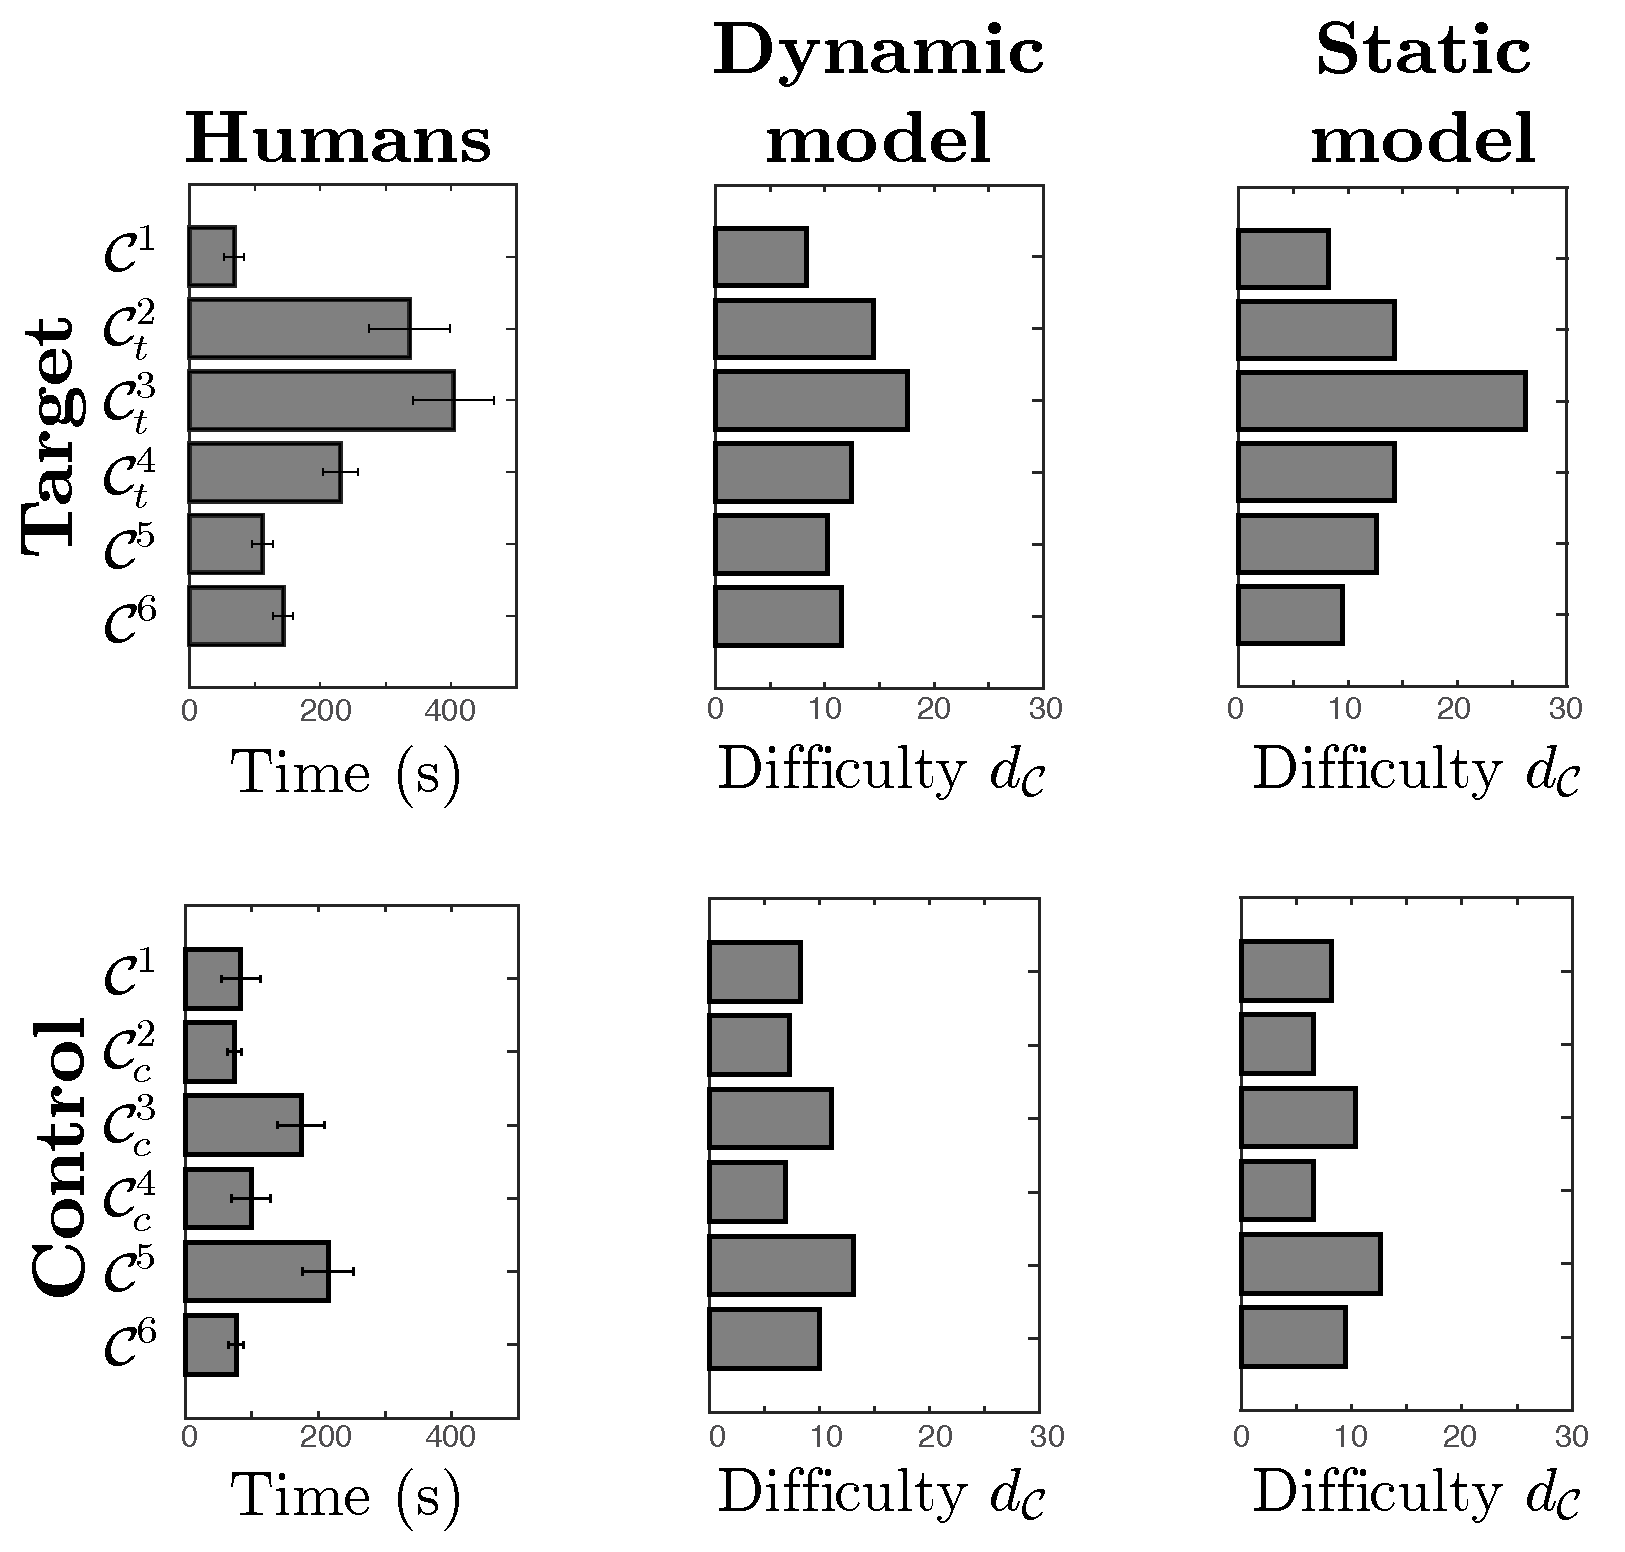
\includegraphics[scale=.30]{results-3.pdf}
      \caption{
      % Learning times and model predictions for target and control groups (see Table~\ref{conceptos} for concept details). The predicted difficulties of each model were calculated using $d_\con$. Error bars are s.e.m.
      Tiempos de aprendizaje y predicciones de modelos para grupos objetivo y control (consultar la Tabla~\ref{conceptos} para obtener detalles de los conceptos). Las dificultades predichas de cada modelo se calcularon utilizando $ d_\con $. Las barras de error son s.e.m.
      }
      \label{results}
\end{figure}

\begin{figure}
        \centering
        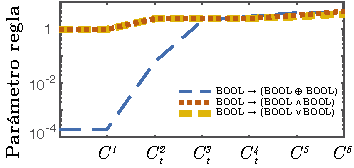
\includegraphics[scale=1]{dirichlet_evol-2.pdf}
        \caption{
        % Evolution of Dirichlet parameters of different rules after each concept experienced by the target group.
        Evolución de los parámetros de Dirichlet de diferentes reglas después de cada concepto experimentado por el grupo objetivo.
        }
       \label{evol}
\end{figure}\santi{aca hay alguna diferencia de nomenclatura de conceptos. Prefier llamarlos $C^1, C^2$, o lo que sea igual a BRM}


% However, the little increment in the $\oxor$ rule after \targetb (see Fig.~\ref{evol}) is sufficient for making the formula $x_{k} \oxor x_{l}$ to have higher relative posterior in the next concepts, making the increment in the parameter of the $\oxor$ rule much greater than before. Additionally, the difficulty inferred by the model is much smaller the second time the concept is presented (compare \targetd and \targetb concepts in Fig.~\ref{results}), since now the posterior is more evenly distributed between long (without $\oxor$) and short (with $\oxor$) formulas (see Eq. \eqref{expected length}). Finally, when the concept \testa is presented, the learner has completely compiled the $\oxor$ rule into her language, ascribing the formulas that use the $\oxor$ operator a much higher posterior probability relative to the long formulas that do not use the $\oxor$ operator. Therefore, the inferred difficulty for \testa is much smaller than those describing previous concepts, almost as simple as concept \targeta (see Fig.~\ref{results}).
Sin embargo, el pequeño incremento en la regla $ \oxor $ después de \targetb (ver Fig.~\Ref{evol}) es suficiente para hacer que la fórmula $x_ {k} \oxor x_{l} $ tenga una probabilidad posterior relativa más alto en los siguientes conceptos, haciendo que el incremento en el parámetro de la regla $ \oxor $ sea mucho mayor que antes. Además, la dificultad inferida por el modelo es mucho menor la segunda vez que se presenta el concepto (comparar los conceptos \targetd y \targetb en la Fig.~\ref{results}), ya que ahora la probabilidad posterior se distribuye más uniformemente entre fórmulas largas (sin $ \oxor $) y fórmulas cortas (con $ \oxor $) (ver la ecuación \eqref{expected length}). Finalmente, cuando se presenta el concepto \testa, el aprendiz\santi{traduje `learner' como `aprendiz'} ha compilado completamente la regla $ \oxor $ en su lenguaje, atribuyendo a las fórmulas que usan el operador $ \oxor $ una probabilidad a posteriori mucho más alta en relación con las fórmulas largas que no usan el operador $ \oxor $. Por lo tanto, la dificultad inferida para \testa es mucho menor que las que describen los conceptos anteriores, casi tan simple como el concepto \targeta (ver Fig.~\ ref{resultados}).

% Finally, the strong $\oxor$ acquired by the target group increases the difficulty of \testb relative to the control group (see Fig. 3). This occurs because there are several formulas of length 9 that use the $\oxor$ operator (around 6000), significantly increasing the expected difficulty of the concept (see Eq. \eqref{expected length}). For the control group, the posterior probability of these formulas is very low, causing a smaller increase in the expected difficulty.
Finalmente, el fuerte $ \oxor $ adquirido por el grupo objetivo aumenta la dificultad de \testb en relación con el grupo de control (ver Fig. 3). Esto ocurre porque hay varias fórmulas de longitud 9 que usan el operador $ \oxor $ (alrededor de 6000), lo que aumenta significativamente la dificultad esperada del concepto (ver ecuación \eqref{expected length}). Para el grupo  control, la probabilidad a posteriori \santi{traduje `posterior' como `probabilidad a posteriori'} de estas fórmulas es muy baja, provocando un menor aumento de la dificultad esperada.

% The previous results point to a competition between different rules in the grammar. In our model, competition between $\oxor$ and the other operators is modulated by the initial relative value of the Dirichlet prior of the $\oxor$ rule, and the overall magnitude of the priors of all rules. The initial $\oxor$ prior measures how useful $\oxor$ should be (relative to the other rules) in order to increase the likelihood of using it in the future. If the $\oxor$ prior is too low relative to the priors of other rules, then formulas with $\oxor$ must be much shorter than formulas without $\oxor$ in order for them to have appreciable posterior and increase the $\oxor$ parameter in Eq. \eqref{Dirichlet}. In our experiment, if the prior is smaller $10^{-12}$ (and 1 for all other rules), then the predictions of the dynamic and static model for the target group are approximately equal: the advantage of using $\oxor$ in the target concepts is not enough to increase the likelihood of using $\oxor$. On the other hand, if the $\oxor$ prior is too high, we cannot model the high difficulty of \targetb for the target group and the high difficulty of \testa for the control group. For example, if the $\oxor$ prior is higher than 0.05 (and 1 for all other rules), the difficulty of \targetb and \targetd are approximately equal (corresponding to the short formula with $\oxor$) and also the difficulties of \testa for control and target groups.
Los resultados anteriores apuntan a una competencia entre diferentes reglas en la gramática. En nuestro modelo, la competencia entre $ \oxor $ y los otros operadores está modulada por el valor relativo inicial de la probabilidad a priori de Dirichlet de la regla $ \oxor $ y la magnitud general de las distribuciones a priori de todas las reglas. La probabilidad a priori inicial del $ \oxor $ mide qué tan útil debería ser $ \oxor $ (en relación con las otras reglas) para aumentar la probabilidad de usarlo en el futuro. Si la probabilidad a priori de $ \oxor $ es demasiado bajo en relación con las distribuciones a priori de otras reglas, entonces las fórmulas con $ \oxor $ deben ser mucho más cortas que las fórmulas sin $ \oxor $ para que tengan un posterior apreciable y aumenten el parámetro de $ \oxor $ en la ecuación \eqref{Dirichlet}. En nuestro experimento, si el valor de la probabilidad a priori es menor $ 10^{- 12} $ (y 1 para todas las demás reglas), entonces las predicciones del modelo dinámico y estático para el grupo objetivo son aproximadamente iguales: la ventaja de usar $ \oxor $ en los conceptos objetivos no es suficiente para aumentar la probabilidad de usar $ \oxor $. Por otro lado, si la probabilidad a priori de $ \oxor $ es demasiado alto, no podemos modelar la alta dificultad de \targetb para el grupo objetivo y la alta dificultad de \testa para el grupo de control. Por ejemplo, si la probabilidad a priori de $ \oxor $ es mayor que 0.05 (y 1 para todas las demás reglas), la dificultad de \targetb y \targetd son aproximadamente iguales (correspondientes a la fórmula corta con $ \oxor $) y también las dificultades de \testa para control y grupos objetivo. \santi{traduje `prior' como `probabilidad a priori'. Tal vez haya una mejor traducción (más corta)}

% The other free parameter that modulates competition is the overall magnitude of the Dirichlet priors, which determines how many times an efficient rule should be encountered before incorporating it. If the magnitude is too high, then observing a useful rule does not significantly change its Dirichlet parameter relative to the others, eliminating from the model the rapid rule acquisition clearly showed by participants. This happens because in Eq. \eqref{Dirichlet} the magnitude of the updates from $t$ to $t+1$ are at most of order $M$, the number of times that operators appear in formulas with high posterior. In our experiment, if all rules have prior equal to 1 and $\oxor$ has 1/1000 we get similar results to the ones in Fig.~\ref{results}, but if all rules have prior equal to 10000 and $\oxor$ has 10 the additions to the $\oxor$ parameter are insignificant, so the dynamic and static models make the same predictions for the target group.
El otro parámetro libre que modula la competencia es la magnitud general de las probabilidades a priori de Dirichlet, que determina cuántas veces se debe encontrar una regla eficiente antes de incorporarla. Si la magnitud es demasiado alta, la observación de una regla útil no cambia significativamente su parámetro de Dirichlet en relación con los demás, eliminando del modelo la rápida adquisición de reglas claramente mostrada por los participantes. Esto sucede porque en la ecuación. \eqref{Dirichlet} la magnitud de las actualizaciones de $ t $ a $ t + 1 $ son como máximo del orden $ M $, el número de veces que los operadores aparecen en fórmulas con probabilidad posterior alta. En nuestro experimento, si todas las reglas tienen una probabilidad a priori igual a 1 y $ \oxor $ tiene una de 1/1000, obtenemos resultados similares a los de la Fig.~\Ref{resultados}, pero si todas las reglas tienen una probabilidad a priori igual a 10000 y $ \oxor $ tiene 10, las adiciones al parámetro de $ \oxor $ son insignificantes, por lo que los modelos dinámico y estático hacen las mismas predicciones para el grupo objetivo.

% In our model a large enough exposure to a concepts will increase the Dirichlet parameters without bounds, progressively decreasing learning flexibility. Although our experiment is not long enough to test it, such inflexibility is very unlikely to be true. For example, in the \lot fitting experiment from~\cite{piantadosi2016logical} they found that human Dirichlet priors for most propositional operators are between 0.3 and 3, instead of orders of magnitude higher (as expected by Eq. \eqref{Dirichlet} after exposure to a large number of concepts). Therefore, a more complete model of lifelong language acquisition should include an extra normalization or forgetting parameter that decreases the overall magnitude of the Dirichlet parameters, preserving the high learning flexibility that we observed in our experiment.
En nuestro modelo, una exposición suficientemente grande a conceptos aumentará los parámetros de Dirichlet sin límites, disminuyendo progresivamente la flexibilidad de aprendizaje. Aunque nuestro experimento no es lo suficientemente largo para probarlo, es muy poco probable que tal inflexibilidad sea cierta. Por ejemplo, en el experimento de ajuste de \lot de~\cite{piantadosi2016logical} encontraron que las probabilidades a priori de Dirichlet para humanos para la mayoría de los operadores proposicionales están entre 0.3 y 3, en lugar de órdenes de magnitud más altos (como esperaba la ecuación \eqref{Dirichlet} después de la exposición a una gran cantidad de conceptos). Por lo tanto, un modelo más completo de adquisición del lenguaje a lo largo de la vida debería incluir un parámetro extra de normalización u olvido que disminuya la magnitud general de los parámetros de Dirichlet, preservando la alta flexibilidad de aprendizaje que observamos en nuestro experimento.

% \section{Discussion}
\section{Discusión}

% \par We measured the subjective difficulty that participants experience when learning a sequence of concepts. To explain this subjective difficulty, we resource to propositional logic as a  base description language. In the target group we experimented with concepts which can be succinctly described in the base language {\em that also contains an extra operator $\oxor$} for exclusive disjunction but that needed necessarily longer descriptions over the base language (where this operator is absent). On the contrary, the control group is exposed to concepts where $\oxor$ does not help to achieve succinctness.
Medimos la dificultad subjetiva que experimentan los participantes al aprender una secuencia de conceptos. Para explicar esta dificultad subjetiva, recurrimos a la lógica proposicional como lenguaje de descripción base. En el grupo objetivo, experimentamos con conceptos que pueden describirse sucintamente en el lenguaje base {\em que también contiene un operador adicional $ \oxor $} para la disyunción exclusiva pero que necesita necesariamente descripciones más largas sobre el lenguaje base (donde este operador está ausente). Por el contrario, el grupo de control está expuesto a conceptos donde $ \oxor $ no ayuda a lograr la descripciones más concisas.

% Learning times are consistent with the hypothesis that participants in the target group smoothly adopt the $\oxor$ as a new primitive of their \lot in order to absorb the concepts they have been exposed to, with no more incentive than decreasing the expected complexity of future concepts. We do not claim that participants have learned the $\oxor$ operator defined by any specific formula using the previous operators, however, their \lot seems to have constructed an operation that matches the semantics of the exclusive or in order to compress such patterns of data and identify them more efficiently.
Los tiempos de aprendizaje son consistentes con la hipótesis de que los participantes en el grupo objetivo adoptan sin problemas el $ \oxor $ como una nueva primitiva de su \lot para absorber los conceptos a los que han estado expuestos, sin más incentivo que disminuir la complejidad esperada de futuros conceptos. No afirmamos que los participantes hayan aprendido el operador $ \oxor $ definido por ninguna fórmula específica usando los operadores anteriores, sin embargo, su \lot parece haber construido una operación que coincide con la semántica de la disyunción exclusiva para comprimir tales patrones de datos e identificarlos de manera más eficiente.

% \par Here, we focus on transfer learning effects when learning sequential concepts that share the same hierarchical structure. We acknowledge, however, that several other transfer learning effects are present in human sequential logical concept learning, such as when subsequent concepts differ in the relevant variables (e.g.\  color lights in our experiment)~\cite{blair2009extremely}, when changing the relevant variables in subsequent exclusive disjunctions~\cite{kruschke1996dimensional}, or when two categories are learned in an interleaved or a focused manner~\cite{carvalho2014putting}. However, unlike superficial knowledge about the task (like the frequency of appearance of different symbols and logical operators in the concept sequence), identifying the latent hierarchical structure of concepts have extremely important computational consequences: it allows for exponentially less complex representations~\cite{bengio2013representation,lake2015human}, maximizing the expected value of future computations within resource-bounded constraints~\cite{gershman2015computational}. In our task, in order to focus primarily on the learning process of the $\oxor$ structure, we randomize variables in each trial, such that other kinds of transitions are averaged out across participants. 
Aquí, nos enfocamos en los efectos del aprendizaje de transferencia al aprender conceptos secuenciales que comparten la misma estructura jerárquica. Sin embargo, reconocemos que varios otros efectos del aprendizaje de transferencia están presentes en el aprendizaje secuencial de conceptos lógicos humanos, como cuando los conceptos posteriores difieren en las variables relevantes (por ejemplo, luces de color en nuestro experimento)~\cite{blair2009extremely}, al cambiar las variables relevantes en disyunciones exclusivas subsecuentes~\cite{kruschke1996dimensional}, o cuando dos categorías se aprenden de forma intercalada o enfocada~\cite{carvalho2014putting}. Sin embargo, a diferencia del conocimiento superficial sobre la tarea (como la frecuencia de aparición de diferentes símbolos y operadores lógicos en la secuencia de conceptos), identificar la estructura jerárquica latente de los conceptos tiene consecuencias computacionales extremadamente importantes: permite representaciones exponencialmente menos complejas~\cite{bengio2013representation,lake2015human}, maximizando el valor esperado de cálculos futuros dentro de restricciones limitadas por recursos~\cite{gershman2015computational}. En nuestra tarea, para centrarnos principalmente en el proceso de aprendizaje de la estructura $ \oxor $, aleatorizamos las variables en cada ensayo, de modo que se promedien otros tipos de transiciones entre los participantes.

% \par Most \lot studies provide a language that is fixed once trained or inferred over a specific data. We claim that when a specific language beats a second one at fitting some experimental data, what we may be seeing is an effect of prior experience (including from the experiment itself), more than an intrinsic feature of the \lot. This leads to a fundamental difficulty in trying to experimentally uncover what the actual human symbolic substrate of thought is. Experimental results have shown for instance that a grammar with \textit{and, or}, and \textit{not} better explains Boolean concept learning than one with \textit{nand}, despite both being expressively equivalent~\cite{piantadosi2016logical}.  In our view, this cannot be taken to mean anything more than that in the current state of affairs of the world, the \textit{nand} operator is not very useful for compressing information. We have shown that participants can rapidly compile new expressions in their \lot if they begin to be useful, which emphasizes that one cannot simply ignore the order in which concepts are presented to the participant when studying aspects of the \lot.
La mayoría de los estudios de \lot proporcionan un lenguaje fijo una vez que se entrena o se infiere sobre datos específicos. Afirmamos que cuando un lenguaje específico supera a otro en el ajuste de algunos datos experimentales, lo que podemos estar viendo es un efecto de la experiencia previa (incluso del experimento en sí), más que una característica intrínseca del \lot. Esto conduce a una dificultad fundamental para tratar de descubrir experimentalmente cuál es el sustrato simbólico humano real del pensamiento. Los resultados experimentales han demostrado, por ejemplo, que una gramática con \textit{and, pr}, y \textit{not} explica mejor el aprendizaje de conceptos booleanos que una con \textit{nand}, a pesar de que ambas son expresivamente equivalentes~\cite{piantadosi2016logical}. En nuestra opinión, esto no puede significar nada más que en el estado actual de las cosas del mundo, el operador\textit{nand} no es muy útil para comprimir información. Hemos demostrado que los participantes pueden compilar rápidamente nuevas expresiones en su \lot si comienzan a ser útiles, lo que enfatiza que no se puede simplemente ignorar el orden en el que se presentan los conceptos al participante cuando se estudian aspectos de la \lot.

% When Fodor proposed the Language of Thought hypothesis~\cite{fodor1975language}, what he had in mind was a symbolic system we all came equipped with from birth. Stating that this language is in fact always flexible might seem in outright contradiction with Fodor's original idea. In fact, what studies in the \lot literature (including this one) are probably probing is one among many languages in a hierarchy of increasing abstraction. As we progress in life, we find some conceptual summaries useful, and compiled them in a more abstract token. It is even likely that there is no proper hierarchy with sharply defined boundaries between levels, but instead a less organized progression of concepts of increasing abstraction, with thought progressing seamlessly using constructs at different levels. he way for a broader understanding of human cognition.
Cuando Fodor propuso la hipótesis del lenguaje del pensamiento~\cite{fodor1975language}, lo que tenía en mente era un sistema simbólico con el que todos venimos equipados desde que nacimos. Afirmar que este lenguaje es siempre flexible puede parecer en total contradicción con la idea original de Fodor. De hecho, lo que probablemente están investigando los estudios en la literatura de \lot (incluido este) es uno entre muchos lenguajes en una jerarquía de abstracción creciente. A medida que avanzamos en la vida, encontramos útiles algunos resúmenes conceptuales y los compilamos o encapsulamos en una pieza más abstracta. Incluso es probable que no exista una jerarquía adecuada con límites claramente definidos entre niveles, sino una progresión menos organizada de conceptos de creciente abstracción, en donde el pensamiento progresa sin problemas utilizando construcciones en diferentes niveles.

% \section{Conclusion}
\section{Conclusiones}

% We defined a model to measure the subjective difficulty of learning a sequence of concepts. The model updates the grammar production probabilities between concepts and predicts difficulty as the size of compatible formulas weighted by their posterior probability. This learning mechanism allows to simulate the emergence of a new primitive in the language, as it becomes useful to encode the concepts presented so far. The predicted difficulties strongly resembles the pattern of human learning times in a sequence of concepts that required the $\oxor$ operator in order to be efficiently represented.
Definimos un modelo para medir la dificultad subjetiva de aprender una secuencia de conceptos. El modelo actualiza las probabilidades de producción gramaticales entre conceptos y predice la dificultad como el tamaño de fórmulas compatibles ponderado por su probabilidad posterior. Este mecanismo de aprendizaje permite simular la aparición de una nueva primitiva en el lenguaje, ya que resulta útil para codificar los conceptos presentados hasta ese momento. Las dificultades predichas se asemejan mucho al patrón de los tiempos de aprendizaje humano en una secuencia de conceptos que requirieron el operador $ \oxor $ para ser representados de manera eficiente.